%\documentclass[11pt]{book}
%
%\setlength{\parindent}{0pt}
%\setlength{\parskip}{8pt}
%
%\usepackage{amsmath}
%\usepackage{amssymb}
%\usepackage{hyperref}
%
%\renewcommand*{\thefootnote}{\fnsymbol{footnote}}
%
%\setcounter{chapter}{0}
%
%\begin{document}
%
%\section*{A Levelized Comparison of \\ Pulsed and Steady-State Tokamaks}
%
%\let\cleardoublepage\relax \tableofcontents \newpage

\chapter{Introducing Fusion Reactors}

The goal of fusion energy research is to build a profitable nuclear reactor. It has long been joked though that fusion power will always be 20-50 years away. This paper lays a framework for exploring reactor space for functional, efficient designs -- based on the last half-century of the world's experiments. Due to the speed and simplicity of the model, hundreds of reactors can be explored in minutes (outpacing the domestic program slightly).

With this proposed model, interesting reactors can be pinpointed long before engineers hit the blueprints. This should help shorten the time till a profitable reactor, as well as illuminate ways to improve modern plasma theory.

\section{Treating Fusion  as a Science}

When people talk about fusion, they usually talk about plasma physics, and when people talk about plasma physics, they often talk about things like: the sun, lightning, and the aurora borealis. Of these three, the sun is the only nuclear reactor. However, the sun can stay on all day because the massive gravity of its fuel source helps keep it self-contained in space. On Earth, this is not possible -- the plasma fuel\footnote{Plasmas are the fourth state of matter after: solids, liquids, and gases. Fundamentally they are gaseous fluids that respond to electric and magnetic fields.} needs to be contained by other means (i.e. with magnets).

\begin{figure}
	\centering
	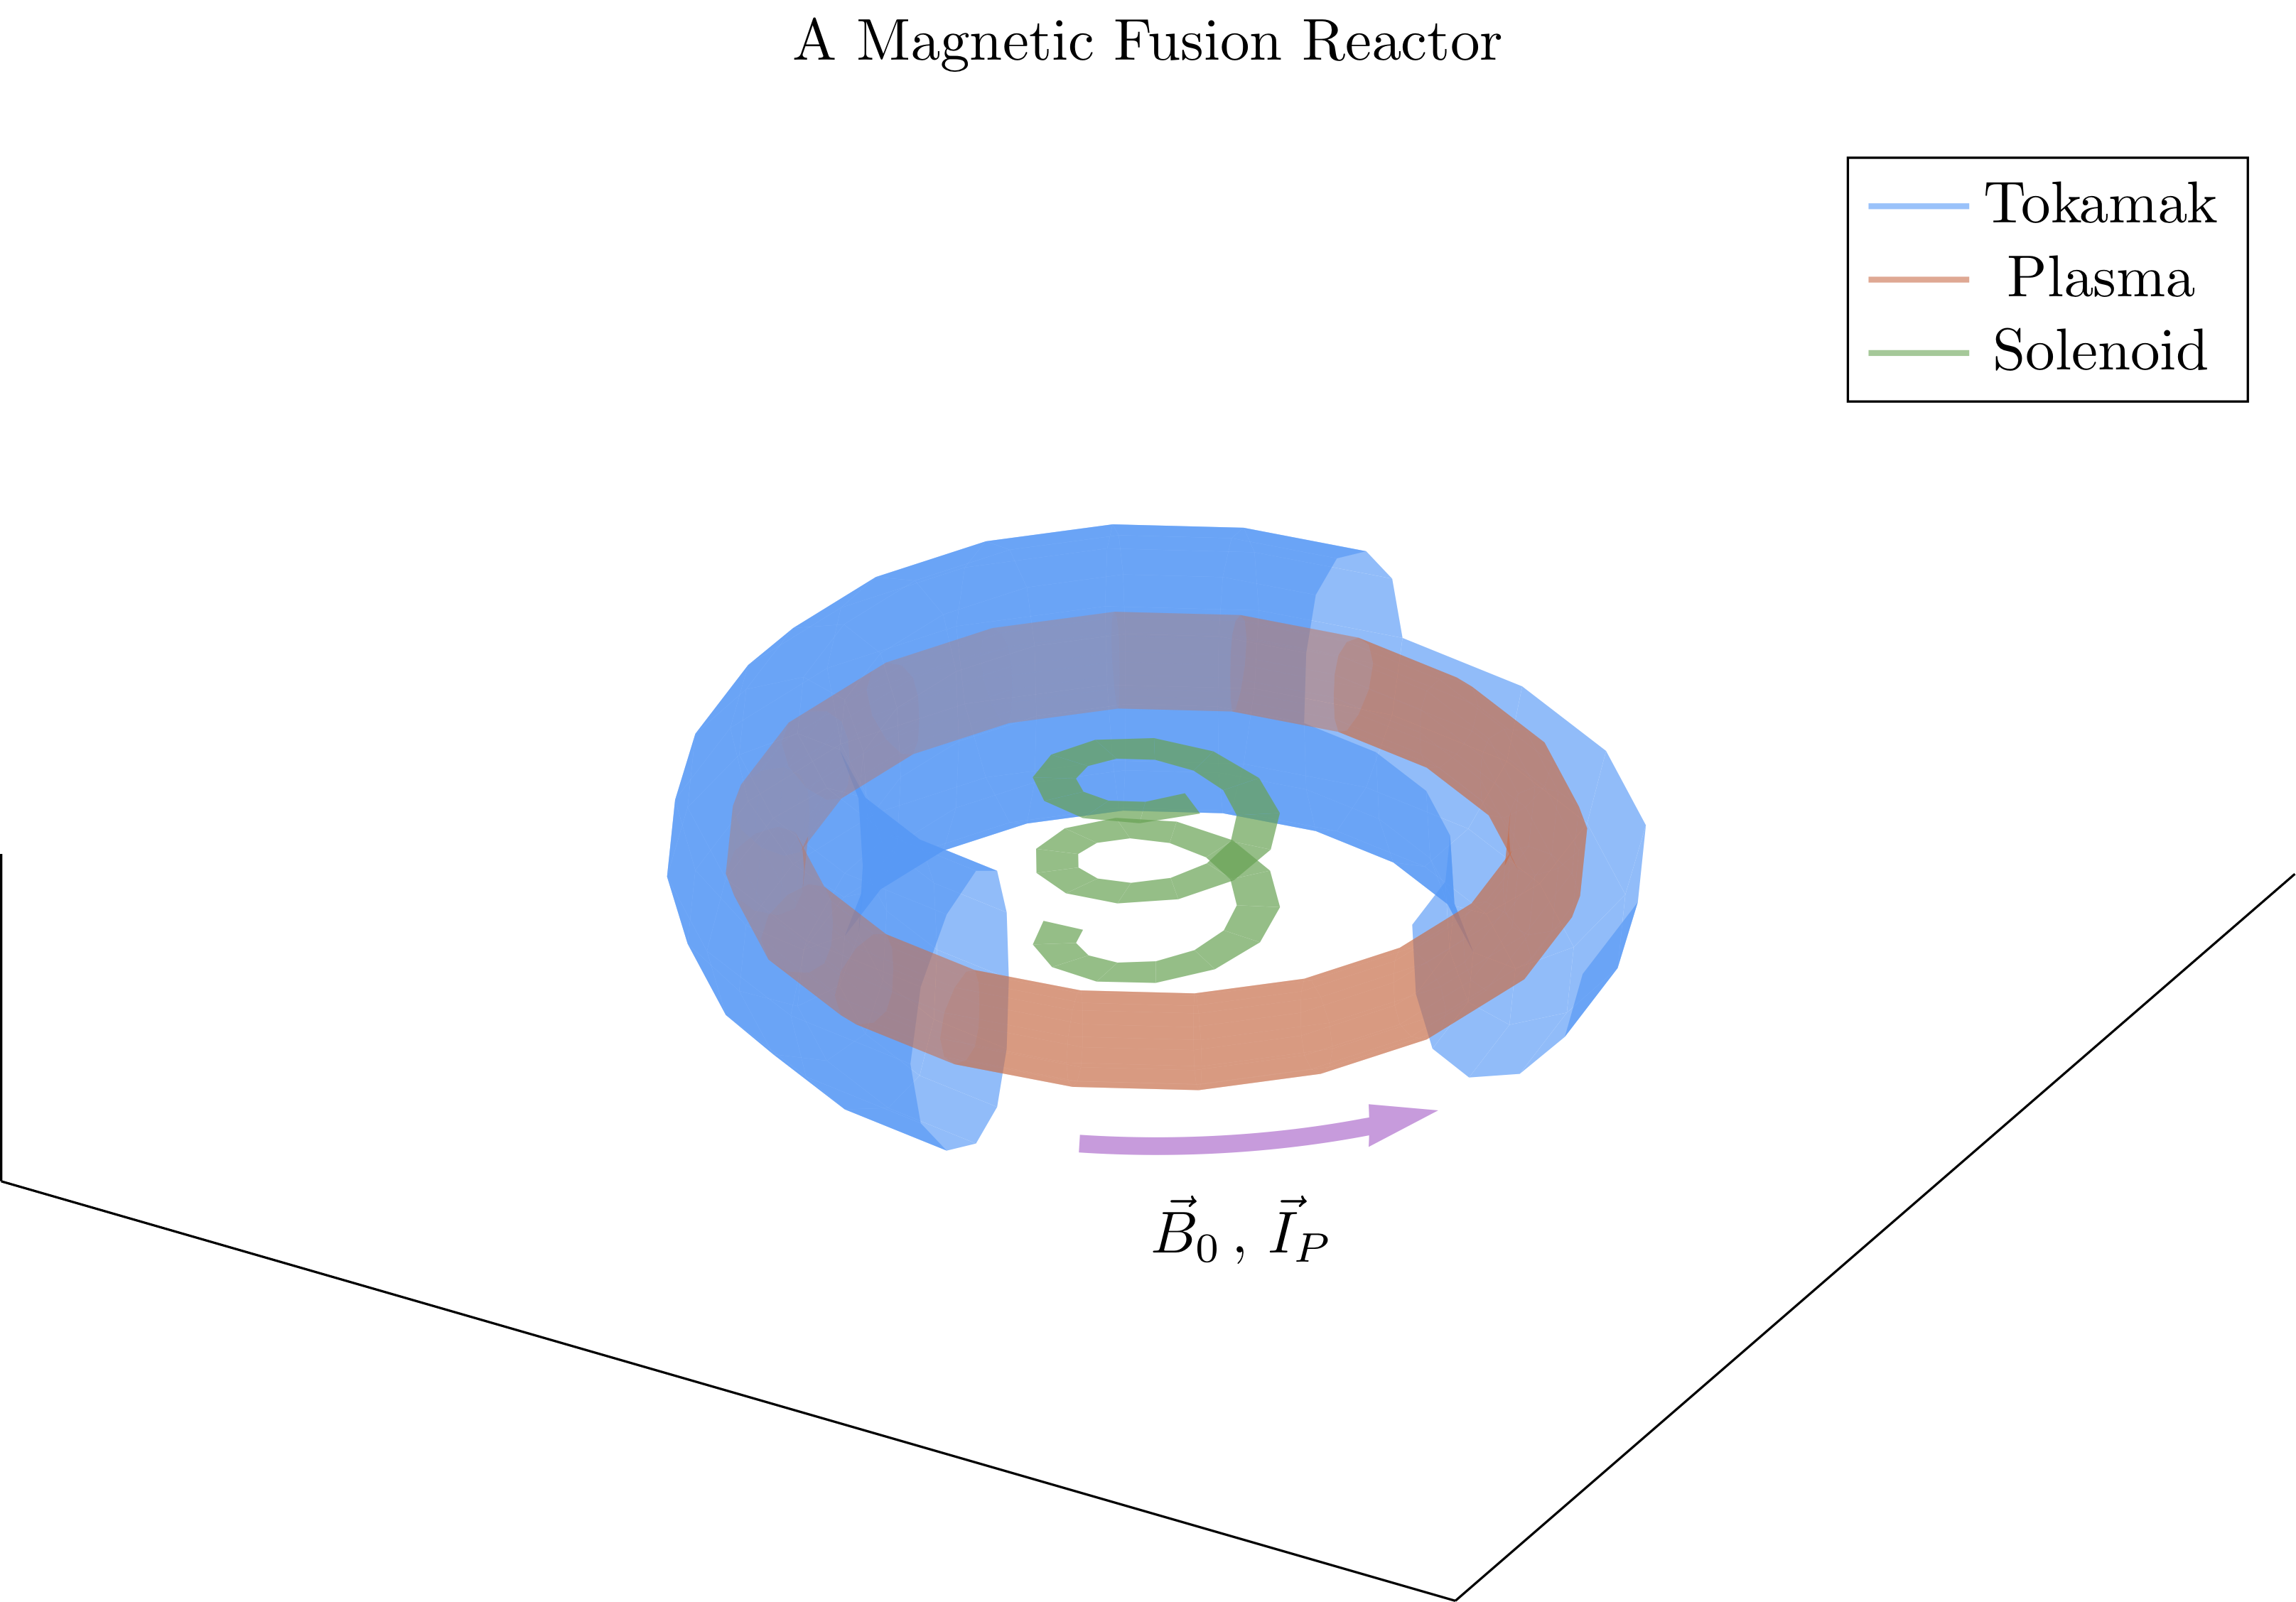
\includegraphics[width=0.75\textwidth]{images/fusion_reactor}
	\caption{Cut-Away of Tokamak Reactor} ~\\
	\small The three main components of a magnetic fusion reactor are: the tokamak structure, the plasma fuel, and the superconducting solenoid at the center.
\end{figure}

A tokamak is one of the leading candidates for a profitable fusion reactor. It shares the shape of a doughnut, using magnets to keep a hula hoop of plasma swirling inside it. The difficulty of keeping this plasma swirling though, is that it does not enjoy being spun too fast or squeezed to hard. Conversely, the tokamak housing the plasma does not like taking too much of a beating or being scaled to T-Rex sized proportions. This sets the stage for tokamak reactor design -- building on the various plasma physics and nuclear engineering constraints of the day. 

One of the most contentious points of building a tokamak, however, is whether it will be run in: pulsed (the European approach \cite{eupulsed}) or steady-state (the United States effort \cite{ussteady}) operation. Here, pulsed operation refers to how a reactor is turned on and off periodically -- around ten times a day. Whereas, steady state machines are meant to be left on nearly the entirety of their 50-year campaigns.

\begin{figure}
	\centering
	\begin{adjustbox}{width=0.75\textwidth}
		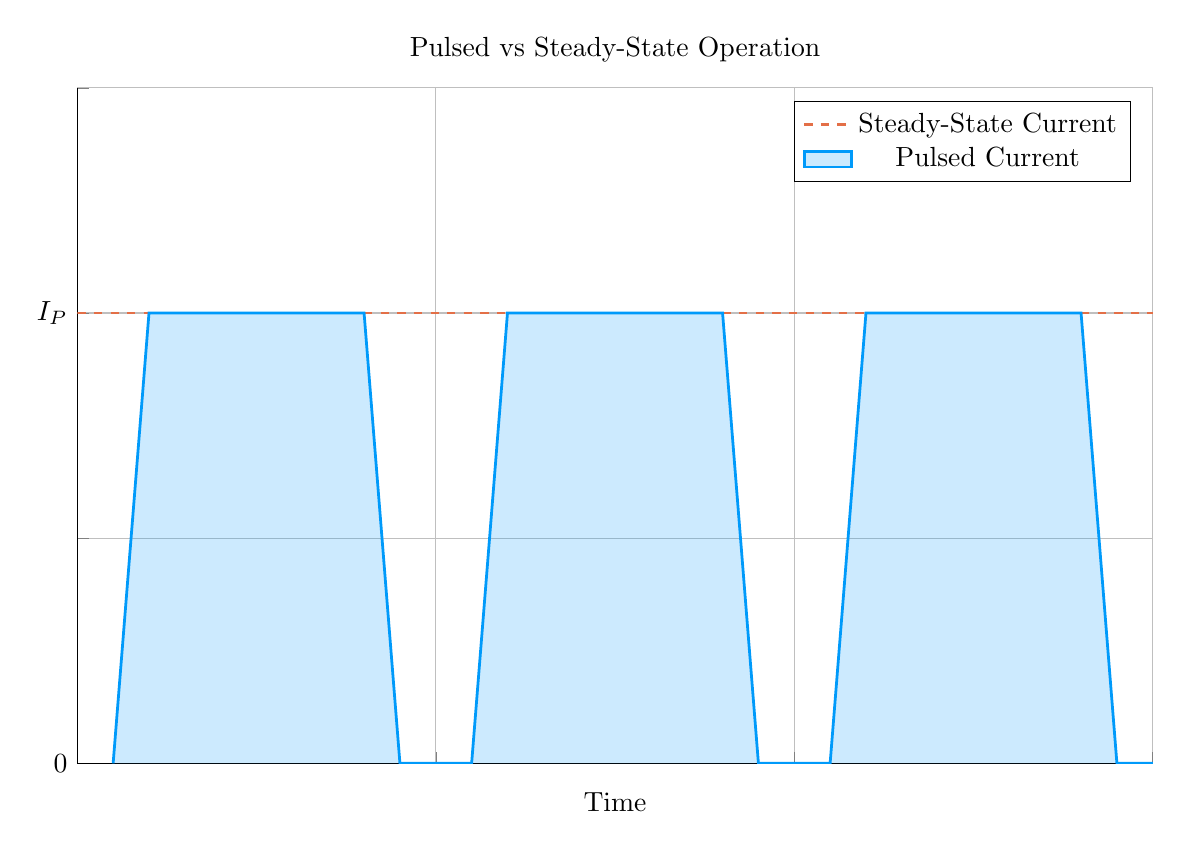
\begin{tikzpicture}[]
\begin{axis}[height = {101.6mm}, ylabel = {}, title = {Pulsed vs Steady-State Operation}, xmin = {0}, xmax = {30}, ymax = {1.5}, xlabel = {Time}, {unbounded coords=jump, scaled x ticks = false, xticklabel style={rotate = 0}, xmajorgrids = true, xtick = {10,20,30}, xticklabels = {}, xtick align = inside, axis lines* = left, scaled y ticks = false, yticklabel style={rotate = 0}, ymajorgrids = true, ytick = {0.0,0.5,1.0,1.5}, yticklabels = {0,,$I_P$,}, ytick align = inside, axis lines* = left,     xshift = 0.0mm,
    yshift = 0.0mm,
    axis background/.style={fill={rgb,1:red,1.00000000;green,1.00000000;blue,1.00000000}}
}, ymin = {0}, width = {152.4mm}]\addplot+ [color = {rgb,1:red,0.88887350;green,0.43564919;blue,0.27812294},
draw opacity=1.0,
line width=1,
dashed,mark = none,
mark size = 2.0,
mark options = {
    color = {rgb,1:red,0.00000000;green,0.00000000;blue,0.00000000}, draw opacity = 1.0,
    fill = {rgb,1:red,0.88887350;green,0.43564919;blue,0.27812294}, fill opacity = 1.0,
    line width = 1,
    rotate = 0,
    solid
}]coordinates {
(0.0, 1.0)
(2.0, 1.0)
(NaN, NaN)
(8.0, 1.0)
(12.0, 1.0)
(NaN, NaN)
(18.0, 1.0)
(22.0, 1.0)
(NaN, NaN)
(28.0, 1.0)
(30.0, 1.0)
};
\addlegendentry{Steady-State Current}
\addplot+ [color = {rgb,1:red,0.00000000;green,0.60560316;blue,0.97868012},
draw opacity=1.0,
line width=1,
solid,mark = none,
mark size = 2.0,
mark options = {
    color = {rgb,1:red,0.00000000;green,0.00000000;blue,0.00000000}, draw opacity = 1.0,
    fill = {rgb,1:red,0.00000000;green,0.60560316;blue,0.97868012}, fill opacity = 1.0,
    line width = 1,
    rotate = 0,
    solid
},fill = {rgb,1:red,0.00000000;green,0.60560316;blue,0.97868012}, fill opacity=0.2,area legend]coordinates {
(1, 0)
(2, 1)
(8, 1)
(9, 0)
(11, 0)
(11, 0)
(12, 1)
(18, 1)
(19, 0)
(21, 0)
(21, 0)
(22, 1)
(28, 1)
(29, 0)
(31, 0)
};
\addlegendentry{Pulsed Current}
\end{axis}

\end{tikzpicture}

	\end{adjustbox}
%	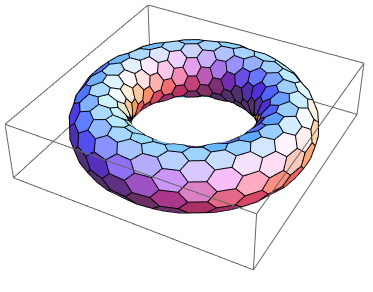
\includegraphics[width=0.85\textwidth]{images/test_image}
	\caption{Comparison of Pulsed and Steady-State Current} ~\\
	\small Inside a pulsed reactor, current is ramped up and down several times a day -- with breaks in-between. Steady state reactors are meant to stay on for weeks, months, or years.
\end{figure}

These two modes of operation, \emph{pulsed} and \emph{steady-state}, greatly influence the design through the current balance equation (derived later). What this means practically is tokamaks need current to spin their plasma hoops at some required speed and this current has to come from somewhere. Luckily, the plasma naturally enjoys spinning and provides some assistance through the bootstrap current. The remaining current must then be produced by external means.

The source of external current drive is what distinguishes pulsed from steady-state devices. Steady-state devices provide the required current assistance either through lasers or particle beams -- this paper's model focuses on a type of laser assistance called lower-hybrid current drive (LHCD). \cite{jeff} Pulsed machines, on the other hand, rely on inductive sources -- which by definition require cycles of charging and discharging several times a day.

The goal of this document is to show that pulsed and steady-state operation are actually two sides of the same coin. This yields the simple conclusion that a single comprehensive model can run both modes at the flip of a switch. It even opens the opportunity of a hybrid reactor that exists somewhere between the two.

\section{Treating Fusion as a Business}

Plasmas may be interesting, but that is not why countries build billion dollar research experiments. The ultimate goal of fusion research is to develop an energy resource that competes with coal and other base-load power sources (e.g. from hydroelectric and nuclear fission power plants). The problem is plasmas are chaotic and hard to contain, while tokamaks are expensive and slow to build. This perfect match has long put the field's project timeline to that of \emph{fusion never}. \cite{fusionfunding}

\begin{figure}[h]
	\centering
	\begin{adjustbox}{width=0.75\textwidth}
		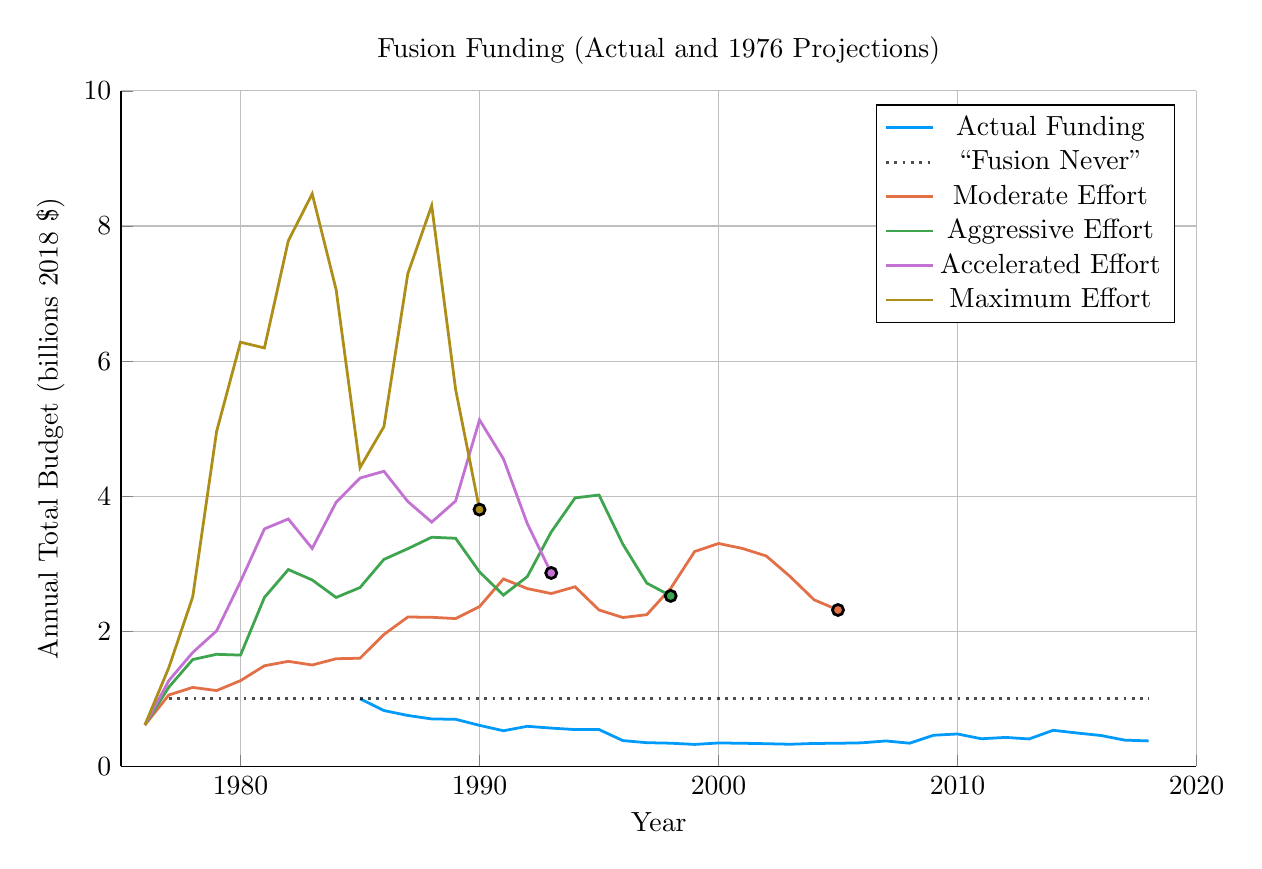
\begin{tikzpicture}[]
\begin{axis}[height = {101.6mm}, ylabel = {Annual Total Budget (billions 2018 \$)}, title = {Fusion Funding (Actual and 1976 Projections)}, xmin = {1975}, xmax = {2020}, ymax = {10}, xlabel = {Year}, {unbounded coords=jump, scaled x ticks = false, xticklabel style={rotate = 0}, xmajorgrids = true, xtick = {1980.0,1990.0,2000.0,2010.0,2020.0}, xticklabels = {1980,1990,2000,2010,2020}, xtick align = inside, axis lines* = left, scaled y ticks = false, yticklabel style={rotate = 0}, ymajorgrids = true, ytick = {0.0,2.0,4.0,6.0,8.0,10.0}, yticklabels = {0,2,4,6,8,10}, ytick align = inside, axis lines* = left,     xshift = 0.0mm,
    yshift = 0.0mm,
    axis background/.style={fill={rgb,1:red,1.00000000;green,1.00000000;blue,1.00000000}}
}, ymin = {0}, width = {152.4mm}]\addplot+ [color = {rgb,1:red,0.00000000;green,0.60560316;blue,0.97868012},
draw opacity=1.0,
line width=1,
solid,mark = none,
mark size = 2.0,
mark options = {
    color = {rgb,1:red,0.00000000;green,0.00000000;blue,0.00000000}, draw opacity = 1.0,
    fill = {rgb,1:red,0.00000000;green,0.60560316;blue,0.97868012}, fill opacity = 1.0,
    line width = 1,
    rotate = 0,
    solid
}]coordinates {
(1985.0, 1.001836)
(1986.0, 0.827367)
(1987.0, 0.754179)
(1988.0, 0.702929)
(1989.0, 0.697497)
(1990.0, 0.608102)
(1991.0, 0.527899)
(1992.0, 0.593976)
(1993.0, 0.567297)
(1994.0, 0.545463)
(1995.0, 0.545963)
(1996.0, 0.382175)
(1997.0, 0.351267)
(1998.0, 0.343818)
(1999.0, 0.325482)
(2000.0, 0.347117)
(2001.0, 0.342814)
(2002.0, 0.336267)
(2003.0, 0.32825)
(2004.0, 0.339832)
(2005.0, 0.342925)
(2006.0, 0.349302)
(2007.0, 0.377075)
(2008.0, 0.343662)
(2009.0, 0.461341)
(2010.0, 0.48051)
(2011.0, 0.409602)
(2012.0, 0.42938)
(2013.0, 0.406833)
(2014.0, 0.534818)
(2015.0, 0.494834)
(2016.0, 0.457833)
(2017.0, 0.389125)
(2018.0, 0.377419)
};
\addlegendentry{Actual Funding}
\addplot+ [color = {rgb,1:red,0.00000000;green,0.00000000;blue,0.00000000},
draw opacity=0.7,
line width=1,
dotted,mark = none,
mark size = 2.0,
mark options = {
    color = {rgb,1:red,0.00000000;green,0.00000000;blue,0.00000000}, draw opacity = 0.7,
    fill = {rgb,1:red,0.00000000;green,0.00000000;blue,0.00000000}, fill opacity = 0.7,
    line width = 1,
    rotate = 0,
    solid
}]coordinates {
(1977, 1)
(2018, 1)
};
\addlegendentry{``Fusion Never''}
\addplot+ [color = {rgb,1:red,0.88887350;green,0.43564919;blue,0.27812294},
draw opacity=1.0,
line width=1,
solid,mark = none,
mark size = 2.0,
mark options = {
    color = {rgb,1:red,0.00000000;green,0.00000000;blue,0.00000000}, draw opacity = 1.0,
    fill = {rgb,1:red,0.88887350;green,0.43564919;blue,0.27812294}, fill opacity = 1.0,
    line width = 1,
    rotate = 0,
    solid
}]coordinates {
(1976.0, 0.61374)
(1977.0, 1.05764)
(1978.0, 1.1695799999999998)
(1979.0, 1.12326)
(1980.0, 1.2699399999999998)
(1981.0, 1.48996)
(1982.0, 1.55558)
(1983.0, 1.5015399999999999)
(1984.0, 1.59418)
(1985.0, 1.6018999999999999)
(1986.0, 1.9531599999999998)
(1987.0, 2.2117799999999996)
(1988.0, 2.2079199999999997)
(1989.0, 2.18862)
(1990.0, 2.36618)
(1991.0, 2.77534)
(1992.0, 2.63252)
(1993.0, 2.55918)
(1994.0, 2.65954)
(1995.0, 2.316)
(1996.0, 2.2040599999999997)
(1997.0, 2.24652)
(1998.0, 2.63638)
(1999.0, 3.18064)
(2000.0, 3.3002999999999996)
(2001.0, 3.2269599999999996)
(2002.0, 3.11502)
(2003.0, 2.8100799999999997)
(2004.0, 2.4665399999999997)
(2005.0, 2.316)
};
\addlegendentry{Moderate Effort}
\addplot+[draw=none, color = {rgb,1:red,0.88887350;green,0.43564919;blue,0.27812294},
draw opacity=1.0,
line width=0,
solid,mark = *,
mark size = 2.0,
mark options = {
    color = {rgb,1:red,0.00000000;green,0.00000000;blue,0.00000000}, draw opacity = 1.0,
    fill = {rgb,1:red,0.88887350;green,0.43564919;blue,0.27812294}, fill opacity = 1.0,
    line width = 1,
    rotate = 0,
    solid
},forget plot] coordinates {
(2005.0, 2.316)
};
\addplot+ [color = {rgb,1:red,0.24222430;green,0.64327509;blue,0.30444865},
draw opacity=1.0,
line width=1,
solid,mark = none,
mark size = 2.0,
mark options = {
    color = {rgb,1:red,0.00000000;green,0.00000000;blue,0.00000000}, draw opacity = 1.0,
    fill = {rgb,1:red,0.24222430;green,0.64327509;blue,0.30444865}, fill opacity = 1.0,
    line width = 1,
    rotate = 0,
    solid
}]coordinates {
(1976.0, 0.61374)
(1977.0, 1.1734399999999998)
(1978.0, 1.5825999999999998)
(1979.0, 1.6598)
(1980.0, 1.6482199999999998)
(1981.0, 2.50128)
(1982.0, 2.9143)
(1983.0, 2.7598999999999996)
(1984.0, 2.50128)
(1985.0, 2.64796)
(1986.0, 3.06484)
(1987.0, 3.2230999999999996)
(1988.0, 3.39294)
(1989.0, 3.3775)
(1990.0, 2.8795599999999997)
(1991.0, 2.5360199999999997)
(1992.0, 2.8100799999999997)
(1993.0, 3.47014)
(1994.0, 3.9757999999999996)
(1995.0, 4.01826)
(1996.0, 3.2887199999999996)
(1997.0, 2.71358)
(1998.0, 2.52444)
};
\addlegendentry{Aggressive Effort}
\addplot+[draw=none, color = {rgb,1:red,0.24222430;green,0.64327509;blue,0.30444865},
draw opacity=1.0,
line width=0,
solid,mark = *,
mark size = 2.0,
mark options = {
    color = {rgb,1:red,0.00000000;green,0.00000000;blue,0.00000000}, draw opacity = 1.0,
    fill = {rgb,1:red,0.24222430;green,0.64327509;blue,0.30444865}, fill opacity = 1.0,
    line width = 1,
    rotate = 0,
    solid
},forget plot] coordinates {
(1998.0, 2.52444)
};
\addplot+ [color = {rgb,1:red,0.76444018;green,0.44411178;blue,0.82429754},
draw opacity=1.0,
line width=1,
solid,mark = none,
mark size = 2.0,
mark options = {
    color = {rgb,1:red,0.00000000;green,0.00000000;blue,0.00000000}, draw opacity = 1.0,
    fill = {rgb,1:red,0.76444018;green,0.44411178;blue,0.82429754}, fill opacity = 1.0,
    line width = 1,
    rotate = 0,
    solid
}]coordinates {
(1976.0, 0.61374)
(1977.0, 1.2699399999999998)
(1978.0, 1.68682)
(1979.0, 2.0071999999999997)
(1980.0, 2.7367399999999997)
(1981.0, 3.51646)
(1982.0, 3.66314)
(1983.0, 3.2269599999999996)
(1984.0, 3.9101799999999995)
(1985.0, 4.269159999999999)
(1986.0, 4.36952)
(1987.0, 3.92176)
(1988.0, 3.6168199999999997)
(1989.0, 3.92948)
(1990.0, 5.1299399999999995)
(1991.0, 4.554799999999999)
(1992.0, 3.59366)
(1993.0, 2.8641199999999998)
};
\addlegendentry{Accelerated Effort}
\addplot+[draw=none, color = {rgb,1:red,0.76444018;green,0.44411178;blue,0.82429754},
draw opacity=1.0,
line width=0,
solid,mark = *,
mark size = 2.0,
mark options = {
    color = {rgb,1:red,0.00000000;green,0.00000000;blue,0.00000000}, draw opacity = 1.0,
    fill = {rgb,1:red,0.76444018;green,0.44411178;blue,0.82429754}, fill opacity = 1.0,
    line width = 1,
    rotate = 0,
    solid
},forget plot] coordinates {
(1993.0, 2.8641199999999998)
};
\addplot+ [color = {rgb,1:red,0.67554396;green,0.55566233;blue,0.09423434},
draw opacity=1.0,
line width=1,
solid,mark = none,
mark size = 2.0,
mark options = {
    color = {rgb,1:red,0.00000000;green,0.00000000;blue,0.00000000}, draw opacity = 1.0,
    fill = {rgb,1:red,0.67554396;green,0.55566233;blue,0.09423434}, fill opacity = 1.0,
    line width = 1,
    rotate = 0,
    solid
}]coordinates {
(1976.0, 0.61374)
(1977.0, 1.46294)
(1978.0, 2.509)
(1979.0, 4.9601)
(1980.0, 6.28022)
(1981.0, 6.1953)
(1982.0, 7.781759999999999)
(1983.0, 8.47656)
(1984.0, 7.059939999999999)
(1985.0, 4.423559999999999)
(1986.0, 5.029579999999999)
(1987.0, 7.2954)
(1988.0, 8.302859999999999)
(1989.0, 5.58156)
(1990.0, 3.8021)
};
\addlegendentry{Maximum Effort}
\addplot+[draw=none, color = {rgb,1:red,0.67554396;green,0.55566233;blue,0.09423434},
draw opacity=1.0,
line width=0,
solid,mark = *,
mark size = 2.0,
mark options = {
    color = {rgb,1:red,0.00000000;green,0.00000000;blue,0.00000000}, draw opacity = 1.0,
    fill = {rgb,1:red,0.67554396;green,0.55566233;blue,0.09423434}, fill opacity = 1.0,
    line width = 1,
    rotate = 0,
    solid
},forget plot] coordinates {
(1990.0, 3.8021)
};
\end{axis}

\end{tikzpicture}

	\end{adjustbox}
%	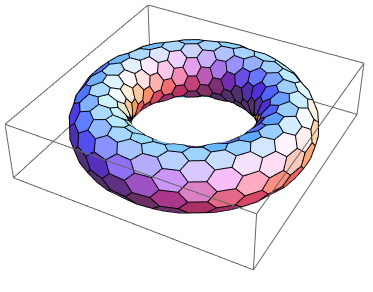
\includegraphics[width=0.75\textwidth]{images/test_image}
	\caption{Fusion Never Funding Timeline} ~\\
	\small Comparison of Projected Timelines of Fusion from 1976 with Actual DOE Budgets. \cite{doe87, doe19} \\ The dotted line is popularly referred to as  ``Fusion Never.'' \cite{fusionnever}
\end{figure}

The major problem with containing a plasma in a reactor is that a plasma does not want to be contained. Since the early days of fusion research, plasmas have often found escape mechanisms. When presented with a magnetic bottle, they found their way out the top. In a tokamak, they attack the outer edges like an overinflated tire-tube. Fusion energy has seemed to remain a Tantalizing effort -- within arms reach, but staunchly guarded by a shroud of instabilities.

The truth is plasmas are extremely chaotic: they show nonlinear behavior in almost everything they do. As of now, no theory or supercomputer-backed code can predict even something so fundamental to design as the movement of energy and particles within a tokamak. As such, the field has adopted several rules of thumb and empirical scalings -- based on the last half century of experiments -- which help one navigate around a plasma's finicky behavior.

The two most widely used rules of thumb within the fusion design community are: the Greenwald density limit and the ELMy H-Mode confinement time scaling law. As such, the model in this document heavily utilizes the two to make a quick running code. These two relations are also why this model -- which happens to be zero-dimensional -- can reproduce with high fidelity the answers from three-dimensional codes, which can take days, weeks, or even months to run!

\begin{figure}
	\centering
	\begin{adjustbox}{width=0.75\textwidth}
		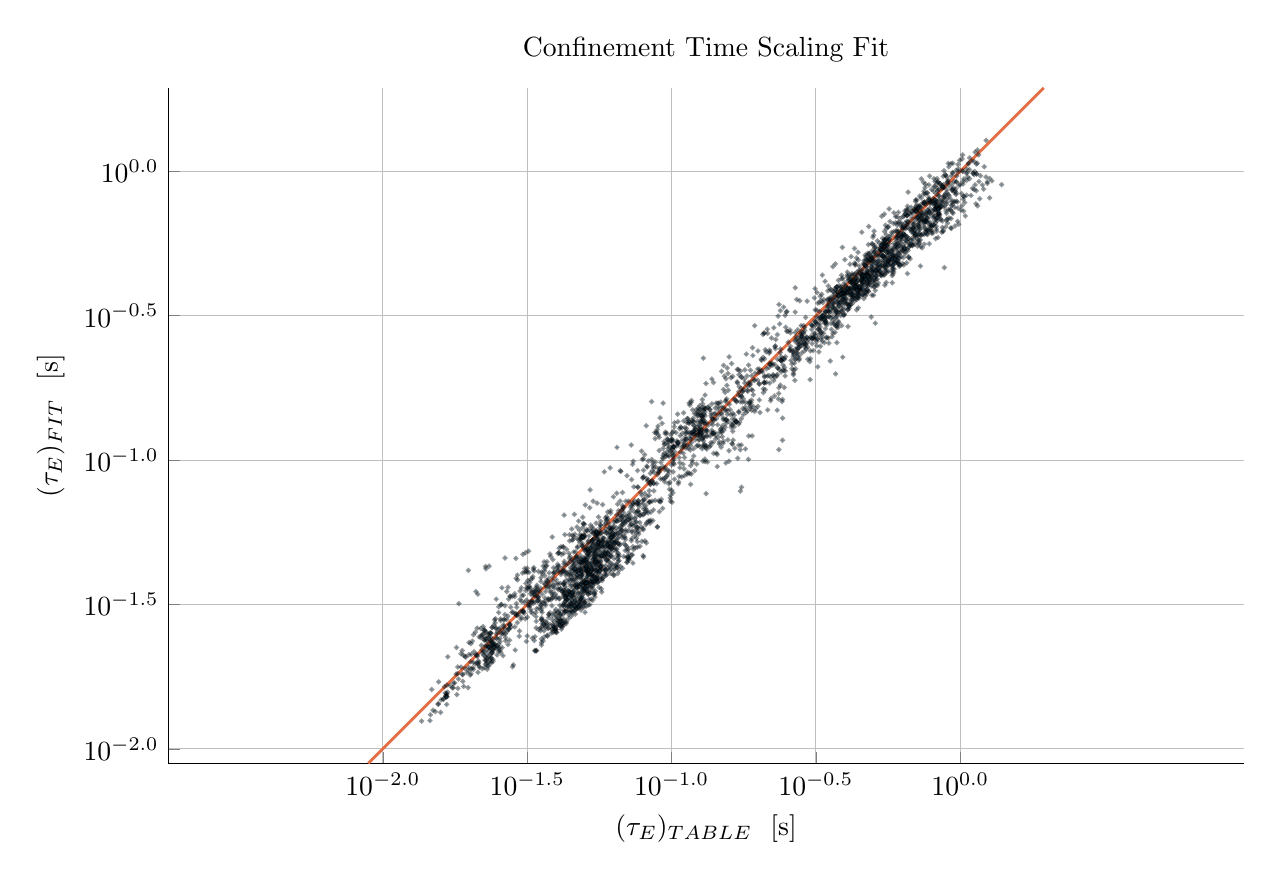
\begin{tikzpicture}[]
\begin{axis}[height = {101.6mm}, axis equal = {true}, ylabel = {$(\tau_E)_{ FIT } \ \ [ \textnormal{s} ]$}, title = {Confinement Time Scaling Fit}, xmin = {0.008904842990761705}, xmax = {1.9473999999999996}, ymax = {1.9473999999999996}, ymode = {log}, xlabel = {$(\tau_E)_{ TABLE } \ \ [ \textnormal{s} ]$}, {unbounded coords=jump, scaled x ticks = false, xticklabel style={rotate = 0}, log basis x=10, xmajorgrids = true, xtick = {0.01,0.03162277660168379,0.1,0.31622776601683794,1.0}, xticklabels = {$10^{-2.0}$,$10^{-1.5}$,$10^{-1.0}$,$10^{-0.5}$,$10^{0.0}$}, xtick align = inside, axis lines* = left, scaled y ticks = false, yticklabel style={rotate = 0}, log basis y=10, ymajorgrids = true, ytick = {0.01,0.03162277660168379,0.1,0.31622776601683794,1.0}, yticklabels = {$10^{-2.0}$,$10^{-1.5}$,$10^{-1.0}$,$10^{-0.5}$,$10^{0.0}$}, ytick align = inside, axis lines* = left,     xshift = 0.0mm,
    yshift = 0.0mm,
    axis background/.style={fill={rgb,1:red,1.00000000;green,1.00000000;blue,1.00000000}}
}, xmode = {log}, ymin = {0.008904842990761705}, width = {152.4mm}]\addplot+[draw=none, color = {rgb,1:red,0.00000000;green,0.60560316;blue,0.97868012},
draw opacity=0.4,
line width=0,
solid,mark = *,
mark size = 0.325,
mark options = {
    color = {rgb,1:red,0.00000000;green,0.00000000;blue,0.00000000}, draw opacity = 0.4,
    fill = {rgb,1:red,0.00000000;green,0.60560316;blue,0.97868012}, fill opacity = 0.4,
    line width = 1,
    rotate = 0,
    solid
},forget plot] coordinates {
(0.048709999999999996, 0.03286927009465151)
(0.047479999999999994, 0.030718782340371346)
(0.056709999999999997, 0.04427687673230967)
(0.06154, 0.040523205193333994)
(0.049249999999999995, 0.031000215657666388)
(0.046439999999999995, 0.03902384637413358)
(0.04536, 0.03366158264691253)
(0.041229999999999996, 0.029311430641277475)
(0.04224, 0.03489492877112558)
(0.05357, 0.03985677848149215)
(0.042449999999999995, 0.030139467297048302)
(0.04393, 0.03525642598465171)
(0.037579999999999995, 0.029115058174186102)
(0.040589999999999994, 0.03552938448965956)
(0.016339999999999997, 0.016414220556232706)
(0.01926, 0.018966660638066977)
(0.014769999999999998, 0.01604916788911629)
(0.020909999999999998, 0.019687625330862386)
(0.014559999999999998, 0.01252323235667468)
(0.016659999999999998, 0.016615842361327)
(0.017099999999999997, 0.016562775820865377)
(0.025429999999999998, 0.024119656293897448)
(0.01834, 0.03183654298531315)
(0.02225, 0.026522518089311862)
(0.02354, 0.023762954142859543)
(0.01883, 0.02190554572449257)
(0.0156, 0.0170549295762654)
(0.01678, 0.020822704009415233)
(0.154, 0.14943255990407037)
(0.17639999999999997, 0.1506224447310805)
(0.7525999999999999, 0.7841653529419872)
(0.7196999999999999, 0.7123510444198007)
(0.7581, 0.7126653992395249)
(0.5971, 0.6636747785042374)
(0.5545, 0.6034081737695671)
(0.5620999999999999, 0.5855426425362842)
(0.7231, 0.611757051674103)
(0.7314999999999999, 0.6000776436052295)
(0.8261999999999999, 0.7332080576221435)
(0.8526999999999999, 0.6874473851854792)
(0.7659999999999999, 0.6249854199535853)
(0.8212999999999999, 0.6647675128338589)
(0.7968, 0.6202645990011652)
(1.1369999999999998, 0.8572954951071405)
(0.8379, 0.709498458538988)
(0.7112999999999999, 0.6481476339591892)
(0.8383999999999999, 0.7100253242029977)
(0.9772, 0.7850517774047457)
(0.6932999999999999, 0.6449986085844157)
(0.7078, 0.5696128161569505)
(0.7666999999999999, 0.6076651618162499)
(0.7231, 0.8218656209469912)
(0.7654, 0.7824204839027497)
(0.8880999999999999, 0.9751544259782554)
(0.9436, 0.987045215482296)
(0.982, 1.0567556111003251)
(1.0659999999999998, 1.0600221351309262)
(1.021, 1.0023421135083617)
(1.037, 0.780421246365204)
(1.0139999999999998, 0.7598649860996711)
(0.9391999999999999, 0.722374477345195)
(0.7876, 0.7737488110528499)
(0.7564, 0.8355652777917266)
(0.8073999999999999, 0.7829615268340135)
(0.6101, 0.662119064106307)
(0.5015, 0.6015695673902948)
(0.7323999999999999, 0.8090796506003152)
(0.6535, 0.7394639493973881)
(0.5972, 0.6975536633839833)
(0.8778999999999999, 0.7874999827504517)
(0.7773, 0.8125562886500788)
(0.6810999999999999, 0.7238692523345119)
(0.6392, 0.701072652615907)
(0.6046999999999999, 0.6507248504722397)
(0.9085, 1.0662323587837632)
(0.746, 0.9171741777262944)
(0.6601999999999999, 0.8477587902173862)
(1.019, 1.1402820961295275)
(0.9123, 1.0371038527895822)
(0.5081, 0.5255375119481419)
(0.7402, 0.6843189302449205)
(0.7313999999999999, 0.6912025500896107)
(1.0779999999999998, 1.1138270195034614)
(0.6314, 0.6309700937894861)
(0.9303999999999999, 0.9647835607071941)
(0.8503, 0.9084098651600415)
(0.8125, 0.8871934724039697)
(0.9943, 1.0920838325900788)
(0.8109999999999999, 0.94316240550339)
(0.7583, 0.9027068941508603)
(0.8357, 0.9197400869136341)
(0.6762999999999999, 0.7509390530838264)
(0.6529999999999999, 0.7031904860947172)
(0.3892, 0.34318485870648646)
(0.34049999999999997, 0.3124029593731834)
(0.45299999999999996, 0.3908324185235881)
(0.44149999999999995, 0.37445805641759866)
(0.5680999999999999, 0.519309036063986)
(0.5427, 0.470258508275619)
(0.3973, 0.3208880474419727)
(0.4023, 0.3620545624474692)
(0.36279999999999996, 0.3723269788644909)
(0.5475, 0.4394327211967968)
(0.3898, 0.37922457801357046)
(0.31279999999999997, 0.303118325347936)
(0.38389999999999996, 0.35281373501460195)
(0.3181, 0.31386085182034285)
(0.7142, 0.6930925801653104)
(0.6252, 0.6626568011479417)
(0.6154999999999999, 0.5263153459242683)
(0.9141999999999999, 0.6902582143865932)
(0.7587999999999999, 0.6215886466745869)
(0.6337999999999999, 0.5997015869390643)
(0.9221999999999999, 0.7382203149764545)
(0.6928, 0.6177290812059213)
(0.7125999999999999, 0.6963967594591091)
(0.21899999999999997, 0.18496435234301067)
(0.20789999999999997, 0.1766203805469118)
(0.26499999999999996, 0.20490261922028621)
(0.4225, 0.34891440428748743)
(0.4118, 0.3421446077261888)
(0.2397, 0.22159945467095882)
(0.26959999999999995, 0.22409261472703068)
(0.3127, 0.2631427459860977)
(0.32389999999999997, 0.2832737570128158)
(0.8515999999999999, 0.9068928303444452)
(0.8177, 0.9220516908419841)
(1.0179999999999998, 1.002889177259622)
(0.5892999999999999, 0.7186483132855688)
(0.9675999999999999, 0.918899482262656)
(0.8809999999999999, 0.4645188486258639)
(1.077, 1.013495270683344)
(0.5667, 0.7415870515780109)
(0.5344, 0.6992580529977903)
(0.5457, 0.7114200487063042)
(0.6599999999999999, 0.568829584256022)
(0.7506999999999999, 0.604323636235005)
(0.7131, 0.5987909231331726)
(0.6576, 0.5815966808550769)
(0.6386, 0.6040200009888924)
(0.4816, 0.6444934910993216)
(0.45589999999999997, 0.6160051006574458)
(0.6427999999999999, 0.7305600248168257)
(0.8285999999999999, 0.7476043736628556)
(0.6534, 0.6544069370264392)
(0.6638999999999999, 0.6723198321350972)
(0.5883999999999999, 0.5629685596654105)
(0.6073999999999999, 0.5947667114406178)
(0.5639, 0.5731530731910407)
(0.6101, 0.6034835968431853)
(0.6638999999999999, 0.5863468310710566)
(0.6346999999999999, 0.5309682418246683)
(0.5062, 0.456996379113654)
(0.6548999999999999, 0.703107054401337)
(0.5526, 0.5545528151553201)
(0.8658999999999999, 0.7858011508612296)
(0.7361, 0.7026740161837454)
(0.734, 0.7080907193345652)
(0.722, 0.7026124938878728)
(0.9287, 1.0629014859458583)
(0.7698999999999999, 0.84074579772222)
(0.8176, 0.8870105921186713)
(0.5843999999999999, 0.5035404234450113)
(0.9373999999999999, 0.8698220688660848)
(0.9337, 0.8623382177770421)
(0.8964, 0.7160170198322513)
(0.7332, 0.9423078640879671)
(0.7831999999999999, 0.963224279565402)
(0.9906999999999999, 0.8952623033567918)
(0.9087, 0.8308130537672082)
(0.7955, 0.8658102097350978)
(0.9360999999999999, 0.9039593399896794)
(0.7863, 0.714131359979918)
(0.8229, 0.740299033130453)
(0.823, 0.760314511413916)
(0.7636999999999999, 0.7163144408463683)
(0.6311, 0.5556779797096207)
(0.6262, 0.6533313908678976)
(0.8946999999999999, 0.9586908006605939)
(0.8576999999999999, 0.7537146014939096)
(0.8473999999999999, 0.7461424250229518)
(0.9255, 0.801575405231461)
(0.8498, 0.7649223531344689)
(0.7823, 0.7268518889656576)
(0.8255999999999999, 0.7470872412684922)
(0.8631, 0.7753860665056598)
(0.7994, 0.728145541191726)
(0.8747999999999999, 0.8208827079316118)
(1.015, 1.1045865073889138)
(1.1609999999999998, 0.9219761380746218)
(0.7623, 0.6715119057586799)
(0.7824, 0.6467686006890678)
(0.5243, 0.564617572937227)
(0.5503999999999999, 0.5783318044105018)
(0.5407, 0.5701439812605221)
(0.5317999999999999, 0.5494542896098417)
(0.5491999999999999, 0.5670933149802504)
(0.5455, 0.5598085924937554)
(0.8478, 0.7018507562099994)
(0.7223999999999999, 0.6570441876740942)
(0.8067, 0.7135500971429034)
(0.7686999999999999, 0.6885128255514706)
(0.7448999999999999, 0.6760240646258281)
(0.7343, 0.6742929760912958)
(0.6597999999999999, 0.7354882011318915)
(0.6793999999999999, 0.7289884081681665)
(0.6546, 0.7051597393592424)
(0.9087999999999999, 0.7368656746766299)
(0.7526999999999999, 0.671806203783079)
(0.7545, 0.8781283223894364)
(0.969, 1.0091726548574242)
(0.9864999999999999, 0.9978820947672817)
(0.9519, 0.8476711232851686)
(0.8273999999999999, 0.778663500363082)
(0.8248, 0.7801934517664398)
(0.6835, 0.6627837535553688)
(0.6928, 0.6114247462326845)
(0.7931999999999999, 0.6269714335560767)
(0.7208, 0.6045147201505461)
(0.6963999999999999, 0.6028585041743847)
(0.8253999999999999, 0.6317543998575686)
(0.6675, 0.5602136085491106)
(0.7319, 0.6026263780884397)
(0.6533, 0.5360321914526158)
(0.564, 0.4904554472531542)
(0.9439, 0.7157171194446946)
(0.7939999999999999, 0.6411620402371146)
(0.8091999999999999, 0.6525781912908896)
(0.7292, 0.5485933677696657)
(0.6357999999999999, 0.503286345980577)
(0.6447999999999999, 0.5185162967617107)
(1.069, 1.0695180372896376)
(0.8583, 0.8908809768320126)
(0.8087, 0.8543034142940075)
(0.8318, 0.9446369769051516)
(0.7786, 0.8979525071302351)
(1.1219999999999999, 0.9996281574893591)
(1.107, 0.9853860242113884)
(1.2109999999999999, 1.0380777356700828)
(1.109, 0.988185626984255)
(0.8967999999999999, 0.7722301840545289)
(0.824, 0.8390911317907782)
(0.8246, 0.7494173273698013)
(0.7246999999999999, 0.6803976433290927)
(0.6926, 0.6607682224597816)
(0.8103999999999999, 0.7710346210832281)
(0.7748999999999999, 0.7325112272388337)
(0.7414999999999999, 0.7062682017319861)
(0.8249, 0.6842066249663288)
(0.8475999999999999, 0.7093971409693103)
(0.7781999999999999, 0.6302194723063099)
(0.7003999999999999, 0.6008831528899192)
(0.6518999999999999, 0.5945976708252837)
(0.7195999999999999, 0.5780911978357602)
(0.7698999999999999, 0.6045774400058568)
(0.6951999999999999, 0.5594902956731888)
(0.6265999999999999, 0.5281946682083224)
(1.0519999999999998, 0.9316449640552941)
(1.011, 0.8373271253227542)
(1.0619999999999998, 0.9564802790915702)
(0.9991, 0.8998058834673238)
(1.1019999999999999, 0.874362127898913)
(0.9502999999999999, 0.7861813492490419)
(1.1929999999999998, 0.8970574608241824)
(1.1409999999999998, 0.9798783118539908)
(1.1389999999999998, 0.981247441890904)
(0.7454, 0.6506062999832742)
(0.7213999999999999, 0.6316980480914915)
(0.7511, 0.6382470829505086)
(1.168, 0.8045488413734408)
(1.1329999999999998, 0.7723998453123871)
(1.2049999999999998, 0.8686731269524)
(0.8418, 0.7105640304650586)
(0.8438, 0.7167529167481481)
(0.8319, 0.6761440014142099)
(0.7971999999999999, 0.647212185326572)
(0.8099999999999999, 0.6507837939912798)
(0.954, 0.7838744415871535)
(1.0279999999999998, 0.8191939822720388)
(1.029, 0.8188141254422304)
(0.9371999999999999, 0.765214397024378)
(1.0219999999999998, 0.9050020965486358)
(1.1449999999999998, 1.0674931488210169)
(1.136, 1.0609598989430766)
(0.9721, 0.9642173576087313)
(0.8966, 0.8641697646781274)
(0.8880999999999999, 0.8373748291165626)
(0.8997999999999999, 0.8442042621804475)
(1.0219999999999998, 0.9220333467704045)
(1.126, 0.897657994702853)
(1.2879999999999998, 0.9272527550966493)
(0.8389, 0.7182547844853155)
(0.9348, 0.7828004050235056)
(1.051, 0.8269739428545848)
(1.0239999999999998, 0.8005745674982954)
(1.158, 1.1412196875478482)
(0.8996, 0.8065770952173787)
(0.9666999999999999, 0.8315473131899693)
(0.8414999999999999, 0.7684067296642498)
(0.8493999999999999, 0.7527319188772996)
(0.8481, 0.7458196646149527)
(0.8429, 0.7423208728716764)
(0.8990999999999999, 0.7842614607464142)
(0.8253999999999999, 0.7485587864344085)
(0.8107, 0.7384132406448961)
(0.8147, 0.7410312659641048)
(0.9854999999999999, 1.0196276084818066)
(1.1469999999999998, 1.1863286392932)
(1.126, 1.1666665208852889)
(0.9404999999999999, 0.8611051902461748)
(0.7303, 0.7213915082892701)
(1.0959999999999999, 1.0877850615898468)
(1.117, 1.0833298051794935)
(1.057, 0.9923729605851154)
(0.9539, 0.9233369235535771)
(1.2289999999999999, 1.2805920757347342)
(0.8688999999999999, 0.8918437252115444)
(0.8352999999999999, 0.8716065387445937)
(0.9081999999999999, 0.9368678123602089)
(0.8755, 0.90002820580841)
(0.8695999999999999, 0.8794079728006472)
(0.8787999999999999, 0.881459737915593)
(0.9007, 0.9104206399267062)
(0.872, 0.8798842972291739)
(0.8658999999999999, 0.8749949687250976)
(0.8429, 0.8633412845042695)
(0.8341, 0.8574697533575164)
(0.7795, 0.80110995309816)
(0.8055, 0.8051314579770487)
(0.7888999999999999, 0.7871440794358052)
(0.7888, 0.78597297922507)
(0.7839999999999999, 0.783736968755363)
(0.8906999999999999, 0.9705362439027034)
(0.8353999999999999, 0.9206177853670467)
(0.9397, 0.9901636819697397)
(0.833, 0.9066645584090964)
(0.7091, 0.7411169895186779)
(0.7263999999999999, 0.7515058392068585)
(0.9071999999999999, 0.9226286568967264)
(0.8681, 0.8888136889786512)
(0.7014999999999999, 0.7549502980032216)
(0.6941999999999999, 0.7414453256597049)
(0.6193, 0.6868705118704591)
(0.7438999999999999, 0.7801456918201667)
(0.6958, 0.7373496835919023)
(0.7162, 0.7545932329675524)
(0.7295999999999999, 0.7653022211346575)
(0.7071, 0.7633267093779594)
(0.7009, 0.79841785676154)
(0.7074999999999999, 0.7960705831433198)
(0.6993999999999999, 0.7869623482126145)
(0.7202, 0.7611057495934285)
(0.7847999999999999, 0.7953466660425729)
(0.7509999999999999, 0.7704143379652046)
(0.6954999999999999, 0.7363969319361924)
(0.6666, 0.7152819454604417)
(0.7485999999999999, 0.7778447754623078)
(0.7101999999999999, 0.7347703554376556)
(0.6983999999999999, 0.7278364728917994)
(0.5580999999999999, 0.4833226862967873)
(0.6591999999999999, 0.5325006454360778)
(0.6224999999999999, 0.507999140907478)
(0.592, 0.4829571034104287)
(0.5678, 0.4750822637133591)
(0.5478999999999999, 0.46940311682153735)
(0.7485999999999999, 0.7775297709191064)
(0.7027, 0.7322537919167466)
(0.7165999999999999, 0.7453502012689315)
(0.7544, 0.7813252510105715)
(0.701, 0.7340106625957865)
(1.0499999999999998, 0.9847941321751483)
(0.7162, 0.7493085145738181)
(0.6687, 0.7135001121348747)
(0.7599999999999999, 0.768274815018355)
(0.7058, 0.7290656456829794)
(0.7031, 0.7275885380278503)
(0.7041, 0.6367181066561843)
(0.688, 0.6354802698552251)
(1.077, 0.943090689087118)
(0.9655999999999999, 0.8715157034912367)
(0.8762, 0.8088387283718785)
(0.8806999999999999, 0.8127564086172461)
(0.5542999999999999, 0.41253102576251693)
(0.5478, 0.4036039372001265)
(0.4941, 0.373031283060472)
(0.5829, 0.512947049410342)
(0.5613999999999999, 0.48664164380957775)
(0.5247999999999999, 0.4527986103525293)
(0.4695, 0.4227065708121077)
(0.48919999999999997, 0.5073610229958332)
(0.6664, 0.5504072752437238)
(0.6019, 0.506184963883185)
(0.5290999999999999, 0.46835384346341935)
(0.6813999999999999, 0.5595253856241379)
(0.5491999999999999, 0.47440537547191425)
(0.5149999999999999, 0.454161051345693)
(0.6145999999999999, 0.5153919313492221)
(0.5720999999999999, 0.48890197499449095)
(0.7011999999999999, 0.5951245600889739)
(0.6801999999999999, 0.5862584147630384)
(0.6436, 0.5779925943174439)
(0.6879, 0.6355711960485161)
(0.7161, 0.6580154715421902)
(0.6805, 0.6403947308683965)
(0.5677, 0.4994502254665087)
(0.6407999999999999, 0.537341813479382)
(0.5336, 0.4735622145714224)
(0.6022, 0.48585628016871496)
(0.5301999999999999, 0.43812776843405565)
(0.5569, 0.4511379734712108)
(0.5309999999999999, 0.4382828143980356)
(0.7189, 0.561283944496514)
(0.6033, 0.49593491486870384)
(0.5882, 0.48791409058918084)
(0.5133, 0.47086714482313546)
(0.6835, 0.5557071339364735)
(0.5457, 0.4595648149111282)
(0.5548, 0.46523133962452173)
(0.47969999999999996, 0.4249658620586939)
(0.4523, 0.415295964493189)
(0.6022, 0.5400209296818028)
(0.5538, 0.5052764641657136)
(0.5436, 0.5055194776119623)
(0.6782999999999999, 0.6163137196828592)
(0.695, 0.6266243673269388)
(0.62, 0.5813674172258797)
(0.6432, 0.5431537583550402)
(0.6287999999999999, 0.5349480622390502)
(0.6376, 0.54586058250559)
(0.5668, 0.4914002086290934)
(0.5511999999999999, 0.47842606650822395)
(0.5179999999999999, 0.4490979395028368)
(0.4926, 0.43740028298001615)
(0.45459999999999995, 0.4189036373559835)
(0.6536, 0.5941545657972782)
(0.5829, 0.5349527992919924)
(0.18815494499765392, 0.1581399078244611)
(0.2146061814556331, 0.19572896069781145)
(0.16599999999999998, 0.13799498658430565)
(0.18969999999999998, 0.14876546786696357)
(0.1833, 0.1482841294703696)
(0.1813, 0.14622039951602703)
(0.17729999999999999, 0.14361309282173648)
(0.1793, 0.14932396239540086)
(0.16018654635778376, 0.14375168149593862)
(0.23608148464163825, 0.20618864049175167)
(0.15090505517866634, 0.13993845766847318)
(0.16462308753545907, 0.14319802218703614)
(0.22867658825412063, 0.2432843316035902)
(0.15437048917401763, 0.19150835096181462)
(0.204407884525842, 0.2234568824525145)
(0.3385921358212541, 0.25515688094639516)
(0.30803062388011077, 0.2920590580475614)
(0.3698439872088892, 0.1989826760084809)
(0.3020055284361583, 0.1900834656284462)
(0.391747288185283, 0.22739364529660014)
(0.18722432262129804, 0.1513418397949884)
(0.35449272544635624, 0.220335621447283)
(0.23145587735894824, 0.1958237725659035)
(0.22568075547813332, 0.1966426493637936)
(0.12419999999999999, 0.12535236963339896)
(0.1362, 0.12116477109254274)
(0.1686, 0.18668565060566708)
(0.2571, 0.24065324034899624)
(0.14309999999999998, 0.10574864224466833)
(0.1001, 0.07861924902447287)
(0.1394, 0.11523665402006138)
(0.13169999999999998, 0.11054302384899538)
(0.1679, 0.16024914750084338)
(0.1679, 0.1592375423514523)
(0.1379, 0.1269124989160874)
(0.13759999999999997, 0.13474346567467413)
(0.15669999999999998, 0.11752104464678922)
(0.1634, 0.11731413030603775)
(0.1513, 0.11615944954854357)
(0.1641, 0.1342046675569159)
(0.1324, 0.11202070716494673)
(0.144, 0.10455225164776064)
(0.08367999999999999, 0.07550572887234856)
(0.08138, 0.06960465607403137)
(0.07985999999999999, 0.06790024415870552)
(0.06914, 0.06133434654420463)
(0.07455999999999999, 0.0659594636095902)
(0.06749, 0.059094960344554005)
(0.07956999999999999, 0.06457109181522346)
(0.07042, 0.06434532605690742)
(0.1243, 0.11740776302358609)
(0.1098, 0.10570841747417169)
(0.11209999999999999, 0.10998875997985506)
(0.12769999999999998, 0.10957807347983331)
(0.10719999999999999, 0.1065573371040371)
(0.13019999999999998, 0.11151703529901563)
(0.11929999999999999, 0.10336177621901224)
(0.18949999999999997, 0.16142608123554003)
(0.13319999999999999, 0.0985814769637825)
(0.122, 0.12133203045600598)
(0.13249999999999998, 0.12167416353208241)
(0.1772, 0.16311084283670516)
(0.11599999999999999, 0.12343156692499643)
(0.118, 0.12364896689819536)
(0.14439999999999997, 0.13258051012966407)
(0.08478999999999999, 0.06604715398119469)
(0.06265, 0.05571638354031536)
(0.06549999999999999, 0.05587664803721788)
(0.07185, 0.06281229971832496)
(0.09925999999999999, 0.07568059816491898)
(0.08231, 0.06687006216262115)
(0.10619999999999999, 0.08785115077712564)
(0.12229999999999999, 0.11192205816899478)
(0.11739999999999999, 0.11521568056327589)
(0.12789999999999999, 0.1567843318502842)
(0.13579999999999998, 0.14986674835019317)
(0.1419, 0.1450258373657531)
(0.16909999999999997, 0.18501546928802198)
(0.17149999999999999, 0.17951957710562474)
(0.1555, 0.1814374863085525)
(0.08192999999999999, 0.060625895818463005)
(0.054299999999999994, 0.04462659847247578)
(0.2382, 0.1819535561143575)
(0.09888999999999999, 0.07391663231244197)
(0.124, 0.14509661104394564)
(0.07007999999999999, 0.08833187686319875)
(0.1354, 0.11128291067705666)
(0.08912999999999999, 0.05866212753957971)
(0.09344, 0.10979611752819195)
(0.08574, 0.09185740084703009)
(0.07637999999999999, 0.08068943179070469)
(0.1404, 0.13841888959775664)
(0.09434999999999999, 0.10565360812919727)
(0.08445, 0.08995215787515654)
(0.07651, 0.08056048684717657)
(0.07107, 0.07211752477661636)
(0.06596999999999999, 0.06504025851381419)
(0.06323, 0.06094593014549412)
(0.12, 0.12630414943307358)
(0.1007, 0.10525729084649234)
(0.1108, 0.1020943378561658)
(0.1661, 0.16132082925344174)
(0.1372, 0.14528321511173972)
(0.15119999999999997, 0.1523332546589318)
(0.1488, 0.14590645549660508)
(0.1263, 0.13574445405586816)
(0.16479999999999997, 0.13044837625750083)
(0.1802, 0.15262991045375698)
(0.15419999999999998, 0.13767198793228275)
(0.2344, 0.16286922831246586)
(0.1619, 0.13198012828918207)
(0.1316, 0.1276676250276773)
(0.1719, 0.13525220987281406)
(0.1177, 0.09988977043209674)
(0.1011, 0.07701041806885227)
(0.1016, 0.09769656334934149)
(0.2014, 0.16156529514473916)
(0.12619999999999998, 0.1453260279389522)
(0.1273, 0.14152422005247894)
(0.10569999999999999, 0.11434661903762405)
(0.1306, 0.1680125891907873)
(0.1319, 0.13503314008427944)
(0.1026, 0.10687459020159086)
(0.09519999999999999, 0.09412923196453649)
(0.08876999999999999, 0.08283955952603496)
(0.10229999999999999, 0.08588833148769484)
(0.08658999999999999, 0.08299779138044373)
(0.12799999999999997, 0.14134838261978305)
(0.10079999999999999, 0.10946905609261658)
(0.09147999999999999, 0.09369943456869442)
(0.08574999999999999, 0.08482791867206357)
(0.08084, 0.0767519431544391)
(0.07662, 0.07222614911256207)
(0.1523, 0.19536945325599323)
(0.11299999999999999, 0.13487967435723913)
(0.10949999999999999, 0.11143501760664376)
(0.09051, 0.09340434624717418)
(0.08438999999999999, 0.08268489965566242)
(0.07891999999999999, 0.07556694845270819)
(0.07379999999999999, 0.07096169353245259)
(0.1397, 0.18575095007051093)
(0.13799999999999998, 0.14010775280450505)
(0.1104, 0.11206507718092389)
(0.102, 0.09676166903886248)
(0.09311, 0.08600781045736207)
(0.08688, 0.07826153594175268)
(0.08052999999999999, 0.07301355683925279)
(0.1487, 0.1442582464317744)
(0.1137, 0.11263854088300114)
(0.09999999999999999, 0.0962223851675817)
(0.09147999999999999, 0.08616202229912978)
(0.08366, 0.07830055417672487)
(0.07941999999999999, 0.0721875693170648)
(0.07307, 0.0675705560076057)
(0.143, 0.13914318897713676)
(0.23379999999999998, 0.31531076056144025)
(0.19399999999999998, 0.29205931398123475)
(0.149, 0.20306944284381495)
(0.09272999999999999, 0.13401719596726916)
(0.08355, 0.0716089079690666)
(0.09022, 0.07228247460420813)
(0.09165, 0.07174064320583198)
(0.11389999999999999, 0.13914314602381422)
(0.1133, 0.13923921674291376)
(0.11889999999999999, 0.1397352499217919)
(0.1568, 0.19945630712290494)
(0.156, 0.2085005358684465)
(0.1306, 0.09881166008611196)
(0.1283, 0.09913341046916643)
(0.08012999999999999, 0.07302668206755579)
(0.06458, 0.06144775295643559)
(0.08765999999999999, 0.07256126399136432)
(0.05644, 0.05559868896061745)
(0.06917999999999999, 0.06275059588936908)
(0.061579999999999996, 0.058396471040249004)
(0.07954, 0.07048587142644203)
(0.1114, 0.11994745431276213)
(0.1113, 0.11733327502135991)
(0.1148, 0.13484774445886444)
(0.11049999999999999, 0.11437476436659133)
(0.10729999999999999, 0.13021477026161207)
(0.1225, 0.13606696165153784)
(0.1157, 0.15513167323708593)
(0.11499999999999999, 0.13411837835876708)
(0.1306, 0.14213468350709502)
(0.08935, 0.08915179338374941)
(0.11009999999999999, 0.14576047007944345)
(0.1278, 0.1619777264626628)
(0.11689999999999999, 0.15853225680858268)
(0.1243, 0.12387254013383525)
(0.1234, 0.14767466023768622)
(0.1273, 0.127599209482771)
(0.11199999999999999, 0.11785537828827053)
(0.13229999999999997, 0.1268143883172406)
(0.12069999999999999, 0.12856174969577555)
(0.1263, 0.13531885730621823)
(0.12649999999999997, 0.1235050552789202)
(0.1498, 0.12054317047255599)
(0.1419, 0.12202374495418274)
(0.12819999999999998, 0.11819378475482076)
(0.1293, 0.1197207947117362)
(0.1249, 0.1320341256906147)
(0.1119, 0.12530666859701617)
(0.12079999999999999, 0.1175727963826226)
(0.1204, 0.12404401900584305)
(0.15419999999999998, 0.16117819943343953)
(0.15519999999999998, 0.1630004223267142)
(0.149, 0.12447480533003696)
(0.1815, 0.23294309109366615)
(0.1515, 0.2128608494637006)
(0.15819999999999998, 0.22787106445763292)
(0.23679999999999998, 0.29618766989262024)
(0.1482, 0.15871540189049393)
(0.1704, 0.16791245305450714)
(0.1541, 0.15959671783996715)
(0.1457, 0.1433583512001976)
(0.1629, 0.14532409688704132)
(0.1392, 0.12337134064185833)
(0.1377, 0.1240380342864336)
(0.1618, 0.11436185846084809)
(0.1304, 0.10081951424495947)
(0.1729, 0.10855438062534839)
(0.12209999999999999, 0.09685894331856996)
(0.09917, 0.0720708881226102)
(0.13179999999999997, 0.07655681296476237)
(0.10039999999999999, 0.07154353600621864)
(0.19299999999999998, 0.18986364317050522)
(0.15849999999999997, 0.1559406980770874)
(0.2203, 0.1607446930750097)
(0.1851, 0.12123867726350177)
(0.17099999999999999, 0.14743911231994888)
(0.1596, 0.14955493831854305)
(0.15419999999999998, 0.09773120055026036)
(0.16909999999999997, 0.2061243181784032)
(0.17029999999999998, 0.2058381027830356)
(0.1606, 0.19290619953642732)
(0.1022, 0.13045114095945723)
(0.09720999999999999, 0.1125395501329079)
(0.1992, 0.23890615900756107)
(0.09857999999999999, 0.08380725082730994)
(0.08400999999999999, 0.0836857170876031)
(0.07471, 0.06121716742820579)
(0.060759999999999995, 0.060182296774004926)
(0.09648, 0.11853897362627272)
(0.10049999999999999, 0.11797322686773393)
(0.11059999999999999, 0.09326023592393005)
(0.102, 0.10089694561208583)
(0.11639999999999999, 0.0957494494183482)
(0.10619999999999999, 0.10201496245161465)
(0.1402, 0.13744893646663867)
(0.1284, 0.13797694791841408)
(0.09651, 0.10670447338174062)
(0.08660999999999999, 0.09403021636813678)
(0.07813999999999999, 0.07734075393518643)
(0.1283, 0.12482444828543321)
(0.1196, 0.12295895913744047)
(0.08606, 0.09579042147664807)
(0.0823, 0.09464568864104099)
(0.056609999999999994, 0.05967258031319823)
(0.055209999999999995, 0.05388213282227408)
(0.1161, 0.11225766369562562)
(0.10869999999999999, 0.11699912494083614)
(0.14839999999999998, 0.1109136505090462)
(0.1901, 0.12128013508649073)
(0.16959999999999997, 0.10151304495153544)
(0.1846, 0.10065505375492664)
(0.1802, 0.10928137721748753)
(0.1581, 0.0991190670353167)
(0.144, 0.09497874232346445)
(0.14559999999999998, 0.15747921112760563)
(0.16469999999999999, 0.16280904518476683)
(0.09311, 0.06809312959312291)
(0.2354, 0.10867715161077376)
(0.1132, 0.08940805796206792)
(0.23859999999999998, 0.24265880726016018)
(0.2014, 0.20649899178209827)
(0.2125, 0.23708492761951952)
(0.1987, 0.2067527428125195)
(0.2582, 0.27595496112874146)
(0.2176, 0.23477458786297317)
(0.21509999999999999, 0.2748956590299204)
(0.2112, 0.24127609628614075)
(0.23559999999999998, 0.34572248038156783)
(0.2445, 0.33877484516585993)
(0.20889999999999997, 0.1860324730832509)
(0.14259999999999998, 0.15760892680189537)
(0.1788, 0.1907498251164262)
(0.20259999999999997, 0.20229735213250857)
(0.25049999999999994, 0.2797364122577605)
(0.24869999999999998, 0.28864117170195547)
(0.2324, 0.27200854100824934)
(0.27259999999999995, 0.24095712361087654)
(0.14479999999999998, 0.15727123584741792)
(0.17099999999999999, 0.146311066352737)
(0.25279999999999997, 0.27915593412286555)
(0.16149999999999998, 0.2159785303177128)
(0.2012, 0.1838662699508891)
(0.17479999999999998, 0.19429681993630987)
(0.1795, 0.20546503367693428)
(0.2065, 0.20172375012643864)
(0.18949999999999997, 0.1960774602491867)
(0.2004, 0.20091302365583058)
(0.20509999999999998, 0.2216737122541796)
(0.1913, 0.23034255208373441)
(0.1671, 0.13608055982080755)
(0.2422, 0.16221177390492433)
(0.1674, 0.13579011535793092)
(0.17079999999999998, 0.13322188934623178)
(0.2422, 0.11709623548612105)
(0.1153, 0.08987545119182616)
(0.11699999999999999, 0.08945266735800408)
(0.09839999999999999, 0.07929935971289688)
(0.09126, 0.07188966657454025)
(0.08113, 0.06571471170536555)
(0.2153, 0.1492539132981206)
(0.1573, 0.13627029545931585)
(0.26739999999999997, 0.1888399985041798)
(0.2473, 0.1957211434435336)
(0.18359999999999999, 0.17325295604505397)
(0.2276, 0.21431505378819005)
(0.21, 0.1955367394519443)
(0.2395, 0.22823459423604212)
(0.20989999999999998, 0.19411397518986154)
(0.18769999999999998, 0.20475009474126396)
(0.23789999999999997, 0.23589564766282592)
(0.16269999999999998, 0.1950964585633041)
(0.1712, 0.19775428241515514)
(0.22219999999999998, 0.21696298191216917)
(0.15119999999999997, 0.1756801334185195)
(0.23329999999999998, 0.20840584050079666)
(0.1793, 0.18506052364877812)
(0.12599999999999997, 0.12287744772297488)
(0.2322, 0.14895050290636133)
(0.1488, 0.1286069479697702)
(0.1866, 0.15734728132882891)
(0.24239999999999998, 0.1397956283398731)
(0.1492, 0.12619156829671674)
(0.17459999999999998, 0.08055313390322363)
(0.07780999999999999, 0.06428661312191306)
(0.17309999999999998, 0.07813376266193288)
(0.09726, 0.08947298251455935)
(0.09426999999999999, 0.08620176021989492)
(0.11599999999999999, 0.10834189064266644)
(0.06767999999999999, 0.05991663837471774)
(0.09945, 0.10692611324801736)
(0.10189999999999999, 0.10409600624325935)
(0.08793, 0.098392083176672)
(0.09173999999999999, 0.09819867560781786)
(0.0881, 0.09467620104667158)
(0.07249, 0.06971858881927705)
(0.06788, 0.0687027184850796)
(0.0638, 0.05214911600923483)
(0.06534, 0.051463869151886554)
(0.09065, 0.10798375106622375)
(0.07407, 0.0808089542364699)
(0.06179, 0.05769612546096603)
(0.05411, 0.04153581887795808)
(0.22119999999999998, 0.16352395227295474)
(0.16269999999999998, 0.13885985821041003)
(0.2412, 0.15953996334513368)
(0.12469999999999999, 0.12551071491627808)
(0.10429999999999999, 0.11657304485547855)
(0.08536999999999999, 0.10049365375288266)
(0.1379, 0.19100894797578152)
(0.1316, 0.18428617507449538)
(0.10239999999999999, 0.13470260690029018)
(0.06288999999999999, 0.07463547168385536)
(0.048319999999999995, 0.05326501666698749)
(0.08302999999999999, 0.09928961207224235)
(0.11729999999999999, 0.1608911209872414)
(0.149, 0.15212784864177845)
(0.18619999999999998, 0.159501776903014)
(0.1284, 0.11939956210704208)
(0.1069, 0.09413987192099378)
(0.11639999999999999, 0.0823526920772639)
(0.18769999999999998, 0.15355776611125668)
(0.1991, 0.15356802969542246)
(0.2287, 0.2487537473757535)
(0.22799999999999998, 0.24700230258041972)
(0.2573, 0.28246695327196)
(0.20989999999999998, 0.22387245009083012)
(0.1329, 0.12554558687880552)
(0.1744, 0.1935795424268048)
(0.18259999999999998, 0.19559326244974617)
(0.2296, 0.2617586433112894)
(0.24969999999999998, 0.325551325400114)
(0.2218, 0.26480813246836626)
(0.1762, 0.17231226581412426)
(0.17609999999999998, 0.1732391867863001)
(0.08295, 0.061486957322273585)
(0.07457, 0.06266876380790434)
(0.07491999999999999, 0.059557100094138865)
(0.07762, 0.06083165347186544)
(0.07651, 0.058267780551432426)
(0.06197999999999999, 0.0577665739122182)
(0.08023999999999999, 0.06499986257129406)
(0.07157999999999999, 0.06150372894319572)
(0.058969999999999995, 0.06309751098303848)
(0.057879999999999994, 0.0537416693041645)
(0.05943, 0.0559945728249867)
(0.059489999999999994, 0.056110927753351775)
(0.042769999999999996, 0.0413682676590617)
(0.03992999999999999, 0.04223255836407681)
(0.041949999999999994, 0.04215722867685451)
(0.030529999999999998, 0.0300339743250663)
(0.030889999999999997, 0.02947397056803015)
(0.06823, 0.06578551977634188)
(0.076, 0.07087353087869819)
(0.06670999999999999, 0.06428197312604807)
(0.07608, 0.07057297019238358)
(0.08127999999999999, 0.06800083709642646)
(0.06728999999999999, 0.0636928217502245)
(0.07306, 0.06297451652537106)
(0.06752999999999999, 0.06006982317240965)
(0.06910999999999999, 0.060465931187406174)
(0.06928999999999999, 0.05735393668498113)
(0.08220999999999999, 0.0747742141627103)
(0.07626999999999999, 0.06653152369237965)
(0.07647, 0.07084263327632506)
(0.08672999999999999, 0.08319125798549942)
(0.08442, 0.08237903544761241)
(0.08524999999999999, 0.08435175719029939)
(0.07744, 0.06573756472416)
(0.09222999999999999, 0.07313801529568059)
(0.08127, 0.06667274731113847)
(0.07221, 0.05982258221378274)
(0.07987, 0.057431530113228595)
(0.07948999999999999, 0.05781483279072657)
(0.06624, 0.05873605187005876)
(0.05848999999999999, 0.056514777560105776)
(0.06298, 0.054616873245672465)
(0.07114, 0.062458481246712584)
(0.06460999999999999, 0.06472646920395032)
(0.07349, 0.07080760838201602)
(0.06549999999999999, 0.0667358866509557)
(0.07398999999999999, 0.06999479702397633)
(0.07737999999999999, 0.07055456609076001)
(0.07214999999999999, 0.06875755572867255)
(0.06960999999999999, 0.06402221874244592)
(0.06441, 0.05817662578647154)
(0.07551999999999999, 0.06382065567962092)
(0.056409999999999995, 0.05694452868487799)
(0.049069999999999996, 0.05462344622251885)
(0.056769999999999994, 0.0613293166979812)
(0.0643, 0.05648369630319677)
(0.05003, 0.04561644832449351)
(0.047779999999999996, 0.0454458249419369)
(0.045739999999999996, 0.04455883579969699)
(0.05465999999999999, 0.05709811483935313)
(0.05341, 0.05584938935322688)
(0.05177, 0.05455199940055293)
(0.054509999999999996, 0.055872293106406304)
(0.05721999999999999, 0.05584146162584512)
(0.05463, 0.05454495200713225)
(0.056729999999999996, 0.055769777958188986)
(0.06764999999999999, 0.06744130324281997)
(0.06692, 0.06688479167403714)
(0.06760999999999999, 0.05540813686444543)
(0.06329, 0.05507643268217983)
(0.06741, 0.05707681444000063)
(0.06866, 0.05440513458870319)
(0.06623, 0.054814540457069995)
(0.06273999999999999, 0.05427589673248694)
(0.061489999999999996, 0.05527004413634945)
(0.09483, 0.08408816730522116)
(0.1566, 0.14820472884968763)
(0.1071, 0.12149261299572511)
(0.1544, 0.13423732792755952)
(0.1283, 0.1384880113792176)
(0.1674, 0.1353148892312939)
(0.1288, 0.13462223185340558)
(0.161, 0.12994450526359577)
(0.1296, 0.13412391229788448)
(0.1421, 0.11851028468528989)
(0.1368, 0.11493579083908262)
(0.1058, 0.08407299739730385)
(0.1084, 0.0874438651574127)
(0.1182, 0.09797171038774165)
(0.1533, 0.1301097475804018)
(0.1228, 0.14218157415906343)
(0.1274, 0.14370143720646936)
(0.1309, 0.15090535522437679)
(0.1512, 0.1380979131720662)
(0.1183, 0.1492713170858393)
(0.1628, 0.1259128126265888)
(0.1248, 0.12722005822535085)
(0.1389, 0.13263042694693655)
(0.1238, 0.15099299116711412)
(0.1297, 0.14411230115170373)
(0.1305, 0.15029373076314514)
(0.04847, 0.045675528167181935)
(0.050379999999999994, 0.044873710407074704)
(0.050749999999999997, 0.04370347874497095)
(0.048479999999999995, 0.043710268049808515)
(0.06319, 0.04559195751176136)
(0.06558, 0.0462767281048458)
(0.08398, 0.061558294911051664)
(0.053509999999999995, 0.07211108621196018)
(0.045829999999999996, 0.054330497917725686)
(0.05207, 0.06842122598337619)
(0.04267, 0.05517926052046134)
(0.055799999999999995, 0.06352502091347549)
(0.05014999999999999, 0.05653506342111358)
(0.04858, 0.053194021280888376)
(0.033209999999999996, 0.0419256579194234)
(0.05023, 0.06991059361959831)
(0.058499999999999996, 0.09112585677836395)
(0.05, 0.054876691080469706)
(0.06470999999999999, 0.1107003689262583)
(0.05523, 0.07092388040718704)
(0.05223, 0.07885854706177597)
(0.05328, 0.05298021417670986)
(0.04557, 0.05316400438323801)
(0.06673, 0.09143741016625018)
(0.057699999999999994, 0.07010510549474457)
(0.125, 0.15393784124347562)
(0.1219, 0.14966336400601812)
(0.07651, 0.0668164568452781)
(0.1345, 0.15305308481153276)
(0.1239, 0.1427402497182206)
(0.1379, 0.15655338527902882)
(0.1292, 0.14906937744964177)
(0.1055, 0.08277935187087547)
(0.129, 0.11639524926090943)
(0.1108, 0.0883125771053816)
(0.1068, 0.09786880127191908)
(0.09776, 0.08277728428981354)
(0.1549, 0.13780788842979494)
(0.12019999999999999, 0.09201427058617603)
(0.15309999999999999, 0.14875740563187737)
(0.14159999999999998, 0.15160597098620893)
(0.13229999999999997, 0.10925760692445917)
(0.15799999999999997, 0.10776553068682639)
(0.08238999999999999, 0.08471609723468296)
(0.07942, 0.08669069291724071)
(0.07976, 0.08706498807067349)
(0.04606, 0.06490335310913804)
(0.04245, 0.0645329376800915)
(0.0973, 0.1096947638706353)
(0.09913, 0.10777002997722854)
(0.0956, 0.10370029408131938)
(0.09354, 0.103938547908765)
(0.1181, 0.13665433557444123)
(0.1198, 0.13567655430912065)
(0.1152, 0.13627982776740938)
(0.0491, 0.044348326049970944)
(0.1002, 0.11823277472074821)
(0.105, 0.1443289348743426)
(0.08746, 0.12465286732832695)
(0.09061, 0.11990519779132883)
(0.08893, 0.12516423419670564)
(0.1301, 0.15214869546469234)
(0.1288, 0.2255155183166059)
(0.09348, 0.15759823893015865)
(0.08528, 0.15941684058432107)
(0.12419999999999999, 0.12195065121186409)
(0.12569999999999998, 0.1374565755280349)
(0.1732, 0.20320665960583337)
(0.13959999999999997, 0.12366910099714125)
(0.14109999999999998, 0.12430754552123721)
(0.12409999999999999, 0.12880032982989656)
(0.15059999999999998, 0.11421111664343418)
(0.16549999999999998, 0.10990801564826941)
(0.1709, 0.11262984028705153)
(0.1744, 0.11286867434901504)
(0.1055, 0.11289515934280171)
(0.1283, 0.11198760726025224)
(0.09007, 0.12225868340047104)
(0.11359999999999999, 0.09068171745435977)
(0.1462, 0.11365702623830429)
(0.14639999999999997, 0.11561011062342046)
(0.13649999999999998, 0.1123931461778589)
(0.1132, 0.12509873540612407)
(0.09333999999999999, 0.09498468586724412)
(0.1251, 0.1116942826507943)
(0.1304, 0.11257872208906217)
(0.1294, 0.12130744690491709)
(0.15019999999999997, 0.13149356252183778)
(0.12589999999999998, 0.12072340901798598)
(0.07783999999999999, 0.06439530806899496)
(0.06775999999999999, 0.06385161520464276)
(0.07626, 0.09201388986727703)
(0.12459999999999999, 0.12714590487008093)
(0.1299, 0.11329191002724368)
(0.13129999999999997, 0.1258856655214462)
(0.09624999999999999, 0.12385402916374029)
(0.09126, 0.140130820406291)
(0.121, 0.13057325091806632)
(0.13849999999999998, 0.13870651374891094)
(0.1142, 0.10995265725315949)
(0.0885, 0.12391235454665024)
(0.06644, 0.09184942445780366)
(0.07164999999999999, 0.06452766437686051)
(0.09735999999999999, 0.11642961582706703)
(0.08070999999999999, 0.10447922483805273)
(0.09434, 0.11360314165418156)
(0.09477999999999999, 0.1135356201973556)
(0.12669999999999998, 0.129975462949832)
(0.08918999999999999, 0.12759437856843164)
(0.109, 0.12380036080640254)
(0.06710999999999999, 0.061818713018713986)
(0.06793999999999999, 0.06133553501580421)
(0.06127, 0.0939913706036707)
(0.121, 0.12771967112435265)
(0.1181, 0.13347411309741714)
(0.11729999999999999, 0.12441504247038145)
(0.12329999999999999, 0.11252768904302743)
(0.16269999999999998, 0.113496351186043)
(0.15589999999999998, 0.14417523179908165)
(0.08771, 0.11859999903705179)
(0.09523, 0.1250204184086543)
(0.11939999999999999, 0.12371081191534117)
(0.11629999999999999, 0.11804369340210522)
(0.10149999999999999, 0.12589039786834094)
(0.10369999999999999, 0.1243916447692094)
(0.1006, 0.12435234256843904)
(0.1399, 0.1055473924806664)
(0.09796999999999999, 0.09163498397751507)
(0.08294, 0.06558549092055614)
(0.07876, 0.10743013860227772)
(0.06841, 0.06845462656277039)
(0.051329999999999994, 0.052057311859872134)
(0.051559999999999995, 0.05254108455984637)
(0.09692999999999999, 0.09217986793723612)
(0.07998, 0.09220581651823166)
(0.06712, 0.0629131318635799)
(0.10099999999999999, 0.09979934695914197)
(0.0861, 0.09800229764971968)
(0.15439999999999998, 0.13860946050196066)
(0.12279999999999999, 0.12210508814948884)
(0.10519999999999999, 0.13584490163220816)
(0.07254, 0.11279009869911553)
(0.11989999999999999, 0.12566268567316524)
(0.11259999999999999, 0.12866661409855143)
(0.1112, 0.1294858844702571)
(0.09941, 0.12232657130752157)
(0.11879999999999999, 0.12601338729640035)
(0.12669999999999998, 0.12426405413897554)
(0.10659999999999999, 0.12845277442343564)
(0.09007, 0.09080934805665608)
(0.09508, 0.1233928617509406)
(0.1294, 0.13667678773620542)
(0.08707, 0.09068530929777574)
(0.1123, 0.12337708199376132)
(0.08198, 0.08639335900843197)
(0.08209999999999999, 0.09523864120856623)
(0.11499999999999999, 0.15767285594551322)
(0.07365999999999999, 0.09907168487830971)
(0.08312, 0.0853612314119027)
(0.09713999999999999, 0.11801143864658041)
(0.07329999999999999, 0.09673907606211848)
(0.06512, 0.063023365872411)
(0.13549999999999998, 0.14955704827553037)
(0.09985, 0.11618485215481959)
(0.09756, 0.11497562639949635)
(0.07457, 0.07221047216387508)
(0.06455999999999999, 0.07674999536987968)
(0.07577999999999999, 0.06590178291411886)
(0.07064999999999999, 0.062222414227090884)
(0.05438, 0.050763778653052906)
(0.06949999999999999, 0.06133222914584153)
(0.05431, 0.051209517320050094)
(0.10079999999999999, 0.10340902849993704)
(0.09806, 0.10294473996353326)
(0.08167999999999999, 0.13155320349132546)
(0.1012, 0.0910179839144466)
(0.09617999999999999, 0.08791569975337975)
(0.08564999999999999, 0.07211056702124978)
(0.10959999999999999, 0.09680617904654507)
(0.12409999999999999, 0.1321602014865297)
(0.14509999999999998, 0.15327592785587155)
(0.12169999999999999, 0.14504819027613808)
(0.07271999999999999, 0.08563754443128341)
(0.1196, 0.1315090384489796)
(0.08979, 0.13122541161208645)
(0.06936999999999999, 0.07202047055670764)
(0.1103, 0.13672581711368698)
(0.104, 0.11185186931596473)
(0.1404, 0.144552147983772)
(0.07677999999999999, 0.07232878130823436)
(0.09974, 0.11698525740125511)
(0.13699999999999998, 0.14243402467920438)
(0.09477, 0.09259434833531666)
(0.08428999999999999, 0.0716081102803995)
(0.1084, 0.12939197175729403)
(0.07917999999999999, 0.10056699555846009)
(0.12549999999999997, 0.1499633270885214)
(0.125, 0.11785049446031891)
(0.1258, 0.12218761772929966)
(0.1176, 0.12024479486655033)
(0.1477, 0.12799981529830304)
(0.12589999999999998, 0.12532263795529228)
(0.12699999999999997, 0.12711880201914286)
(0.11549999999999999, 0.12475342870521901)
(0.13269999999999998, 0.1206690356828618)
(0.1128, 0.11751387493213465)
(0.11499999999999999, 0.11971869826060168)
(0.07988999999999999, 0.1010700832605083)
(0.15339999999999998, 0.17164743250594205)
(0.09304, 0.10172703396904313)
(0.09369999999999999, 0.10115527336607896)
(0.1308, 0.13392963181365516)
(0.1341, 0.13203578883911835)
(0.12749999999999997, 0.1428139857049046)
(0.1175, 0.1370113042456721)
(0.12639999999999998, 0.14261395249606929)
(0.09574999999999999, 0.10327750174654599)
(0.09742999999999999, 0.10404187749552464)
(0.10099999999999999, 0.11045647697951541)
(0.09892999999999999, 0.1103240550664823)
(0.10149999999999999, 0.11176524526508155)
(0.1049, 0.11464659823714847)
(0.102, 0.11144896659771159)
(0.10139999999999999, 0.1115184334913019)
(0.10479999999999999, 0.11514668826256849)
(0.10189999999999999, 0.11074596579716918)
(0.13319999999999999, 0.152134742964813)
(0.1201, 0.1450707224400905)
(0.0953, 0.0871451758926745)
(0.07712, 0.06908716239003389)
(0.08006999999999999, 0.08769541662115697)
(0.06760999999999999, 0.06959655065568175)
(0.1084, 0.11010009805517544)
(0.09054999999999999, 0.09236587853069575)
(0.09047, 0.0908918275722975)
(0.06571999999999999, 0.06171502677099673)
(0.13049999999999998, 0.14669645905988252)
(0.12739999999999999, 0.14902970225305368)
(0.12799999999999997, 0.15208775807296487)
(0.1011, 0.11622942096714987)
(0.09419, 0.11590333943260595)
(0.062139999999999994, 0.043807126805594794)
(0.05121, 0.03758276043879671)
(0.04854, 0.04188928691324043)
(0.058679999999999996, 0.041754403697277835)
(0.051829999999999994, 0.03772453021255255)
(0.056089999999999994, 0.05236381625047371)
(0.09076999999999999, 0.06628979462576573)
(0.07708999999999999, 0.05663764891390501)
(0.052989999999999995, 0.049880565329447395)
(0.08657999999999999, 0.06724796958361724)
(0.07852999999999999, 0.05864519685405708)
(0.057769999999999995, 0.05239550415437296)
(0.08613, 0.061743726336050374)
(0.07558, 0.05363693062268584)
(0.05384, 0.039744205311861486)
(0.04919, 0.03600428248701913)
(0.044059999999999995, 0.03347985370339069)
(0.05755, 0.03826955667730545)
(0.051559999999999995, 0.03512616106470059)
(0.04906, 0.04032372242817625)
(0.058679999999999996, 0.04214444563079101)
(0.05012, 0.037502672969671226)
(0.050129999999999994, 0.042430783157216004)
(0.04822, 0.034792805809842606)
(0.048279999999999997, 0.032619944690633604)
(0.04013, 0.028002041041515307)
(0.04205, 0.029170276562792554)
(0.03738, 0.026162823529597843)
(0.05393, 0.03943172805693677)
(0.050769999999999996, 0.03495612307283419)
(0.043669999999999994, 0.031045632399048853)
(0.04403, 0.031618631445663424)
(0.042699999999999995, 0.029932727265347615)
(0.04108, 0.028925903253109522)
(0.04484, 0.03183738666236927)
(0.045149999999999996, 0.03146721524329628)
(0.039839999999999993, 0.02858424780951381)
(0.0426, 0.02975641390272645)
(0.04357, 0.02996641353096916)
(0.041269999999999994, 0.029193782152619648)
(0.054889999999999994, 0.05500535213193049)
(0.07554999999999999, 0.05591811006975335)
(0.06824, 0.04636280684367296)
(0.05511, 0.04672160286737354)
(0.07113, 0.04584180889427859)
(0.06291, 0.04152720570189643)
(0.054419999999999996, 0.045428123478448955)
(0.06992999999999999, 0.04612361683254559)
(0.06449999999999999, 0.04242120362059848)
(0.061919999999999996, 0.04807160682356552)
(0.07135, 0.045762491094245426)
(0.06363999999999999, 0.04219806322929389)
(0.052, 0.048372279638101104)
(0.07269999999999999, 0.0468040440484844)
(0.06595999999999999, 0.041570472489462135)
(0.05107999999999999, 0.047183085073742595)
(0.07082, 0.0461554492235355)
(0.0629, 0.04006546620834503)
(0.06649999999999999, 0.04287181171264254)
(0.07622999999999999, 0.05837251483801267)
(0.07612999999999999, 0.05215117266301809)
(0.07103999999999999, 0.04759241413313047)
(0.06299999999999999, 0.052817145211616214)
(0.08087, 0.052506486127834665)
(0.07494999999999999, 0.04977898525649905)
(0.056459999999999996, 0.04891705048708967)
(0.07626999999999999, 0.04993263731360597)
(0.07773999999999999, 0.050343045793943254)
(0.07164, 0.06610173472165022)
(0.07299, 0.05615105030368495)
(0.06177, 0.04940751143085813)
(0.06467999999999999, 0.052188354754795545)
(0.07018999999999999, 0.04884134712167059)
(0.052899999999999996, 0.051741716695579455)
(0.07347, 0.05018394405510633)
(0.07013, 0.04421800868229376)
(0.08453999999999999, 0.0617390727633646)
(0.07072999999999999, 0.04529772441151242)
(0.055659999999999994, 0.05451464652476719)
(0.07002, 0.0443650578957311)
(0.05218999999999999, 0.04964667672770208)
(0.08178999999999999, 0.051640094402335475)
(0.07128, 0.045052511376517)
(0.051089999999999997, 0.04874524801561931)
(0.08947, 0.05871229255121658)
(0.06763999999999999, 0.04219320039650211)
(0.07361, 0.05932933487413711)
(0.07380999999999999, 0.04899247538083112)
(0.05916999999999999, 0.03988049695301668)
(0.045739999999999996, 0.03075691624554024)
(0.05014999999999999, 0.035401936689860816)
(0.033449999999999994, 0.023700887298799177)
(0.053309999999999996, 0.032676177975323885)
(0.047099999999999996, 0.03080356662595087)
(0.050699999999999995, 0.03595772068320578)
(0.052719999999999996, 0.033020284032847846)
(0.05067, 0.031184906998317417)
(0.050649999999999994, 0.037656117203829845)
(0.05425, 0.03442624362513712)
(0.05212, 0.03159101870740787)
(0.054439999999999995, 0.035188185934650985)
(0.04645, 0.030224786461125842)
(0.0573, 0.03494551090327198)
(0.048549999999999996, 0.030257084736934982)
(0.04747, 0.04135021016473731)
(0.06317999999999999, 0.03982508027185115)
(0.053959999999999994, 0.0346268854209517)
(0.05143, 0.03427530371566186)
(0.04686, 0.03120614023043205)
(0.056549999999999996, 0.038287530588219355)
(0.048279999999999997, 0.032958921992933446)
(0.053439999999999994, 0.037585052989652805)
(0.039209999999999995, 0.026514308280023078)
(0.05409, 0.037412048857159125)
(0.046639999999999994, 0.03088282794362106)
(0.07297999999999999, 0.05693901026043227)
(0.057769999999999995, 0.046046079564715486)
(0.06492999999999999, 0.043174389389974886)
(0.053149999999999996, 0.03624914998591414)
(0.050219999999999994, 0.03225742769689555)
(0.048229999999999995, 0.03088307422218342)
(0.054299999999999994, 0.0335587098052626)
(0.049749999999999996, 0.031003527657185174)
(0.057109999999999994, 0.0358135779317065)
(0.05143, 0.031485811399370074)
(0.043989999999999994, 0.03761777517924622)
(0.05243, 0.038282480138270826)
(0.04350999999999999, 0.033005142328412534)
(0.08366, 0.07153028553566486)
(0.06323, 0.05176468048260886)
(0.07561, 0.061109348491963394)
(0.06385999999999999, 0.05183748083133759)
(0.054639999999999994, 0.04508115403462853)
(0.07281, 0.05345805985067246)
(0.05962, 0.04523765375910066)
(0.05397, 0.04781061844296936)
(0.06993999999999999, 0.050115911134589464)
(0.05873, 0.04020647496480056)
(0.047779999999999996, 0.04230161759273692)
(0.0658, 0.04488581377727357)
(0.05721, 0.038907659702185675)
(0.04869, 0.03729477101085321)
(0.04049, 0.02974114494857944)
(0.05993999999999999, 0.052024431970484036)
(0.0532, 0.04198675629086556)
(0.043179999999999996, 0.032831826514113836)
(0.057089999999999995, 0.046560287216035466)
(0.04724999999999999, 0.0360910713658527)
(0.042269999999999995, 0.031519775987039554)
(0.049179999999999995, 0.03411621800943581)
(0.047979999999999995, 0.031395409412267636)
(0.04185, 0.026457476863003582)
(0.03143, 0.023559452842022342)
(0.03294, 0.024191193682469768)
(0.03362999999999999, 0.02445319477047692)
(0.05352, 0.04555484255452605)
(0.06036999999999999, 0.04230717245489598)
(0.05898, 0.04092733613909257)
(0.03594, 0.02365069058393874)
(0.0501, 0.037665493374325495)
(0.044899999999999995, 0.029978715337933833)
(0.04405, 0.02834125410198317)
(0.0472, 0.03661553469194371)
(0.04298, 0.03158286755633917)
(0.03859, 0.02805717934692784)
(0.043199999999999995, 0.03378778112236379)
(0.036599999999999994, 0.02763055086580289)
(0.03548, 0.026402444570132584)
(0.045009999999999994, 0.03703011841448374)
(0.045329999999999995, 0.033819895538348514)
(0.03639, 0.02671635397810346)
(0.04436, 0.03496089912997418)
(0.03931, 0.027563793963025496)
(0.04047, 0.026883356729058002)
(0.056429999999999994, 0.04205696457404693)
(0.053689999999999995, 0.037756483483319746)
(0.048769999999999994, 0.033455436981654645)
(0.055729999999999995, 0.04417119268895516)
(0.057519999999999995, 0.041866740635265375)
(0.04887, 0.03385624850789497)
(0.04509, 0.028860198770128964)
(0.04328, 0.027523750313724553)
(0.042129999999999994, 0.026771242589141424)
(0.049539999999999994, 0.036323873064086375)
(0.039119999999999995, 0.026371052445352896)
(0.03961, 0.025854179708570544)
(0.046439999999999995, 0.03301722359260753)
(0.0498, 0.032196506271848294)
(0.043109999999999996, 0.027105912960769706)
(0.07107, 0.049326575054020876)
(0.05538, 0.047189806803314985)
(0.052349999999999994, 0.04296051271539761)
(0.0506, 0.04138058160525018)
(0.05021, 0.037955032628458285)
(0.038669999999999996, 0.02904041064101643)
(0.03943, 0.029289920396264903)
(0.04994, 0.03813699008048943)
(0.03943, 0.0298269422075107)
(0.037489999999999996, 0.028486638285630885)
(0.042499999999999996, 0.035293216474861715)
(0.04323, 0.032761673855646094)
(0.04183, 0.031233257450439693)
(0.05067, 0.041228206190652504)
(0.055299999999999995, 0.04145679364135235)
(0.044879999999999996, 0.03188445303300164)
(0.051579999999999994, 0.048421431277563876)
(0.06305, 0.0491128852804413)
(0.053, 0.03791875345281894)
(0.03585, 0.02786794841954307)
(0.03394, 0.02623117834448156)
(0.035629999999999995, 0.02719573931429382)
(0.036169999999999994, 0.026981104545494138)
(0.035239999999999994, 0.026209812725624077)
(0.03754, 0.029271724901413543)
(0.035989999999999994, 0.027064400898775383)
(0.034629999999999994, 0.025883550055635036)
(0.04742, 0.034555392026848625)
(0.03711999999999999, 0.026894115962422565)
(0.035179999999999996, 0.025633243130909103)
(0.037939999999999995, 0.02695112454493581)
(0.03618, 0.025634398809376048)
(0.04026999999999999, 0.027158340352581127)
(0.036199999999999996, 0.024393946352571364)
(0.05352, 0.0480122407394134)
(0.046259999999999996, 0.036825844828731996)
(0.04248, 0.03214908610941244)
(0.048729999999999996, 0.03604796004122758)
(0.04371, 0.03097584319157523)
(0.061149999999999996, 0.04654581942999267)
(0.05552, 0.04092100373510931)
(0.05021, 0.036408566128837264)
(0.056639999999999996, 0.04160010586103059)
(0.051539999999999996, 0.036650182475572106)
(0.050719999999999994, 0.035366860127939916)
(0.039779999999999996, 0.033184283534412946)
(0.04314, 0.03310277887864934)
(0.042879999999999995, 0.03243468318042962)
(0.03537, 0.028024821149512047)
(0.049839999999999995, 0.03599952802236968)
(0.046139999999999994, 0.031019200946584814)
(0.041229999999999996, 0.02662056645495299)
(0.057019999999999994, 0.039971022591691746)
(0.042199999999999994, 0.027387223798712317)
(0.04153, 0.02595622736579993)
(0.04955, 0.04414358340703178)
(0.04674, 0.04105118737287537)
(0.045599999999999995, 0.04001434425879645)
(0.04416, 0.031072392536260273)
(0.04405, 0.029172748666705474)
(0.04131, 0.026963455158686467)
(0.05307, 0.039939102443030616)
(0.04294, 0.03001031029290522)
(0.04158, 0.028076529913457184)
(0.0482, 0.03715197577398297)
(0.038919999999999996, 0.02660760265621123)
(0.039729999999999994, 0.026371333545799833)
(0.048029999999999996, 0.03178317101479531)
(0.042839999999999996, 0.027559440764451347)
(0.03986, 0.025301463032816076)
(0.04468, 0.03117912257299728)
(0.04246, 0.028088319600306236)
(0.039869999999999996, 0.025883172035342596)
(0.04974, 0.03518875712420223)
(0.04128999999999999, 0.02766285639963346)
(0.0394, 0.025826057456375943)
(0.06481999999999999, 0.04681553415445039)
(0.05177, 0.036144490601876175)
(0.04865, 0.03322277997327565)
(0.049949999999999994, 0.03486760462501651)
(0.045459999999999993, 0.029928672121444885)
(0.04137, 0.026592294764567318)
(0.04631999999999999, 0.032560875988658346)
(0.044379999999999996, 0.02975226714676566)
(0.03938, 0.025910804282523184)
(0.048369999999999996, 0.04230438601068989)
(0.040249999999999994, 0.028629298695145917)
(0.040999999999999995, 0.028013454845046738)
(0.03859, 0.026028936109391845)
(0.05595, 0.040651048020974294)
(0.041229999999999996, 0.028027432153189154)
(0.0389, 0.025306741901049937)
(0.04511, 0.03179471921712473)
(0.040409999999999995, 0.02758606120429414)
(0.03961, 0.026245528738720946)
(0.04622, 0.031238874605723662)
(0.0421, 0.02710348340874567)
(0.040049999999999995, 0.02534401125217854)
(0.046889999999999994, 0.0319978953522729)
(0.04171999999999999, 0.027137277522240388)
(0.039549999999999995, 0.02542923275099463)
(0.05001, 0.04270733316867462)
(0.048819999999999995, 0.03990011739412072)
(0.045689999999999995, 0.035987063029765586)
(0.04321, 0.029963341715362454)
(0.03707, 0.02473775814120398)
(0.035449999999999995, 0.02333833052822582)
(0.051219999999999995, 0.04107922620313101)
(0.04527, 0.03449411206017924)
(0.051879999999999996, 0.04052410773349539)
(0.047479999999999994, 0.03465236967810864)
(0.04946, 0.044796026370465716)
(0.051219999999999995, 0.04061201722646834)
(0.04607, 0.0342101990445086)
(0.06082, 0.058156032358951275)
(0.04373, 0.04037346360760039)
(0.03659, 0.02630697838545053)
(0.035449999999999995, 0.024002694322198023)
(0.0336, 0.02191938919126572)
(0.03723, 0.02456410143773018)
(0.03408, 0.021898138292734654)
(0.044899999999999995, 0.03296744803553329)
(0.03856999999999999, 0.025879606558637504)
(0.033979999999999996, 0.021870743639875723)
(0.04446, 0.03478983476934267)
(0.038799999999999994, 0.02698940111078313)
(0.03365, 0.0217954424138954)
(0.038259999999999995, 0.025160188130300548)
(0.03541, 0.02288524612115034)
(0.05483, 0.038444328645044684)
(0.053259999999999995, 0.03562149453573055)
(0.046819999999999994, 0.030573150028132066)
(0.0658, 0.04693482331225837)
(0.0593, 0.04168611079756195)
(0.043919999999999994, 0.03519771600076149)
(0.04092, 0.02749350239397576)
(0.050859999999999995, 0.04117206139217811)
(0.04131, 0.027568730033184982)
(0.047959999999999996, 0.03357678902249291)
(0.040979999999999996, 0.0268198215038522)
(0.06947999999999999, 0.056322471571686225)
(0.054909999999999994, 0.039180507447196866)
(0.04577, 0.03203521301987455)
(0.0556, 0.039013731832366734)
(0.04545, 0.029684501573588415)
(0.059579999999999994, 0.05181805053938185)
(0.06007, 0.0477458984938311)
(0.05554, 0.04458005175271727)
(0.05964, 0.05127966044286074)
(0.07509999999999999, 0.05710509181060265)
(0.061489999999999996, 0.04648649495034286)
(0.05819, 0.047776706992870226)
(0.06845, 0.05133049158682345)
(0.06064, 0.045837944071215)
(0.04831, 0.041395780527819545)
(0.07251999999999999, 0.05260023656352511)
(0.06391, 0.04306288354098858)
(0.061489999999999996, 0.05054295543010538)
(0.06430999999999999, 0.0492933003922123)
(0.056459999999999996, 0.041483307827431225)
(0.061099999999999995, 0.05000930607013184)
(0.06016, 0.05041839595451042)
(0.05486, 0.04291590518741538)
(0.05298, 0.041550436932967075)
(0.05774, 0.0522281589767972)
(0.06488999999999999, 0.055540984575026375)
(0.05107999999999999, 0.04203718812090458)
(0.05252999999999999, 0.043210938792144875)
(0.06426, 0.04359490611063006)
(0.06478999999999999, 0.042450564314710115)
(0.06741, 0.05393940803467957)
(0.06491, 0.04561127459840459)
(0.05783, 0.03912360915828068)
(0.051179999999999996, 0.0426312349715133)
(0.05712999999999999, 0.04305810278718661)
(0.05508, 0.039529616248591734)
(0.06075, 0.05008749535931189)
(0.06098, 0.04294355608020117)
(0.052439999999999994, 0.03473145039982899)
(0.06388999999999999, 0.05529644883660158)
(0.049769999999999995, 0.0374781494985194)
(0.050809999999999994, 0.03752990586920512)
(0.05255, 0.03992333489812251)
(0.05488, 0.03871516312559054)
(0.05248, 0.03648936403279889)
(0.038509999999999996, 0.03128890418694755)
(0.037919999999999995, 0.029610090390963635)
(0.042499999999999996, 0.031098952591799726)
(0.05916, 0.041532857264628444)
(0.04974, 0.0329483063126124)
(0.055619999999999996, 0.038012113760066385)
(0.04819, 0.031336837068120314)
(0.05227, 0.048454666496922906)
(0.05916999999999999, 0.04644456416277519)
(0.05264, 0.04017404857594558)
(0.056479999999999995, 0.04277695867172708)
(0.058589999999999996, 0.05079197424838071)
(0.0602, 0.05015514312365183)
(0.05635999999999999, 0.04633756360803307)
(0.050929999999999996, 0.04173323455012917)
(0.05522, 0.03754905182335937)
(0.04888, 0.031846553682433436)
(0.05282, 0.04454818747658203)
(0.05245, 0.041161882224101255)
(0.04928, 0.03777537069417967)
(0.05252999999999999, 0.037035319995371456)
(0.05339, 0.03680833694758647)
(0.05479, 0.041400386095808164)
(0.05332, 0.04048032047089661)
(0.050929999999999996, 0.03879256034674798)
(0.06002, 0.052538011386075716)
(0.06046, 0.044779422312630254)
(0.05218999999999999, 0.0376128944515065)
(0.05379, 0.04654214366197547)
(0.05551, 0.03778351219660085)
(0.051359999999999996, 0.03438205656741011)
(0.05925999999999999, 0.047171713083550976)
(0.051449999999999996, 0.040128684667407516)
(0.05606, 0.049878041063484084)
(0.059359999999999996, 0.04500483735227026)
(0.05429, 0.038290772304040745)
(0.060099999999999994, 0.05099245461524577)
(0.05635, 0.044967804581317015)
(0.05298, 0.0417878619726053)
(0.058899999999999994, 0.04728088252737356)
(0.059449999999999996, 0.045017566867429484)
(0.05538, 0.052956042800574206)
(0.05604, 0.05169574481895553)
(0.054669999999999996, 0.049206929902610726)
(0.06045, 0.05514412381137318)
(0.057879999999999994, 0.05027204336303889)
(0.054549999999999994, 0.04742557092488681)
(0.056209999999999996, 0.052535114271623336)
(0.06269, 0.05754602530210281)
(0.05465, 0.05121905861529514)
(0.061489999999999996, 0.0668489892266253)
(0.05862, 0.05967367024187677)
(0.054689999999999996, 0.05493740662994372)
(0.05925, 0.060682410016612884)
(0.05542999999999999, 0.05536244826631737)
(0.05343, 0.05303310781504308)
(0.05434, 0.04430983054107062)
(0.0554, 0.04211920770580433)
(0.050199999999999995, 0.0374338675473437)
(0.03739, 0.03309692417162335)
(0.03387999999999999, 0.02968209716822948)
(0.038669999999999996, 0.03409328513752852)
(0.04285, 0.03400357319125994)
(0.04103, 0.0313985267936527)
(0.05014999999999999, 0.03750884283566652)
(0.06538, 0.044511402466800985)
(0.046169999999999996, 0.030214160297030477)
(0.05626, 0.04334666908089799)
(0.07057, 0.04626667129860035)
(0.05175, 0.03290730440448738)
(0.0382, 0.03278209847144525)
(0.07311999999999999, 0.0470269977484591)
(0.05386, 0.03422438947102727)
(0.060169999999999994, 0.06269833996380637)
(0.06311, 0.05917343865820327)
(0.05737, 0.05263915237303688)
(0.04883, 0.043354986922602076)
(0.051579999999999994, 0.04167475482578621)
(0.04597, 0.03495427684517097)
(0.048929999999999994, 0.04504091425663451)
(0.05663, 0.046937655108107046)
(0.052099999999999994, 0.040174957000100285)
(0.040499999999999994, 0.03733563038602567)
(0.042429999999999995, 0.03549677962595195)
(0.040929999999999994, 0.03320789765877802)
(0.054099999999999995, 0.04871548769637523)
(0.055029999999999996, 0.04133114481814371)
(0.05092, 0.036641925161548176)
(0.04690999999999999, 0.041184548703789924)
(0.046529999999999995, 0.03804736772054051)
(0.042089999999999995, 0.03375303942293149)
(0.037939999999999995, 0.03540797312961206)
(0.04844999999999999, 0.041914336608437935)
(0.051039999999999995, 0.037568714996609166)
(0.04471, 0.03014750947860926)
(0.03351, 0.03440662557935258)
(0.03813999999999999, 0.03476954998348969)
(0.03634999999999999, 0.03236559526246643)
(0.036239999999999994, 0.03736189360112195)
(0.03881999999999999, 0.0381570503955528)
(0.03779, 0.03648970053762369)
(0.03985, 0.03727699665227257)
(0.038799999999999994, 0.03345127248367704)
(0.035649999999999994, 0.029691019501746584)
(0.053489999999999996, 0.04300030245324201)
(0.06910999999999999, 0.04867428601906883)
(0.04786, 0.03232269245875938)
(0.04999, 0.04144444820205272)
(0.050289999999999994, 0.0360723947600714)
(0.04609, 0.032244482728131525)
(0.05586, 0.050802854988832066)
(0.05513, 0.038872733870573405)
(0.055659999999999994, 0.05087725372305442)
(0.07698999999999999, 0.055432650261195246)
(0.05959, 0.04001553205517576)
(0.0518, 0.04688060558559667)
(0.07447999999999999, 0.05458704419645025)
(0.061649999999999996, 0.0421482768796164)
(0.049049999999999996, 0.035493182901452286)
(0.06509, 0.04045751394646205)
(0.050159999999999996, 0.02970807814016159)
(0.055479999999999995, 0.05298923861873267)
(0.06589999999999999, 0.05067097476609811)
(0.05916, 0.043187979054619796)
(0.060759999999999995, 0.058340575702210955)
(0.061309999999999996, 0.056825050388284656)
(0.051739999999999994, 0.047990064291929674)
(0.02872, 0.021991151350571118)
(0.05567999999999999, 0.05600382183293284)
(0.05116999999999999, 0.04415535435910399)
(0.039749999999999994, 0.030400027044893297)
(0.04781, 0.032413782405142075)
(0.055119999999999995, 0.04820939803164962)
(0.060669999999999995, 0.044337518604464984)
(0.044919999999999995, 0.031035606412003307)
(0.045219999999999996, 0.04217874449844669)
(0.054959999999999995, 0.04065656884779951)
(0.04688, 0.03178931623615448)
(0.07088, 0.05694654337189137)
(0.05739, 0.04316363905567389)
(0.05565, 0.03921162167194618)
(0.04752, 0.031019807127883933)
(0.050609999999999995, 0.03869459333360339)
(0.040409999999999995, 0.029689160966617098)
(0.051329999999999994, 0.04194649926197363)
(0.054189999999999995, 0.037961792608831556)
(0.04915, 0.03491641494908949)
(0.04452, 0.03846494689119722)
(0.04999, 0.032104251314690996)
(0.056659999999999995, 0.04274354736297203)
(0.05227999999999999, 0.037961002841612766)
(0.04672, 0.0335418028724764)
(0.053419999999999995, 0.03822814811420505)
(0.05610999999999999, 0.03625793704847974)
(0.046459999999999994, 0.029274393440629005)
(0.047029999999999995, 0.039875433967434516)
(0.06224, 0.043241106786234364)
(0.049609999999999994, 0.031860700377524066)
(0.047499999999999994, 0.03927883260618694)
(0.05214, 0.034685204006533354)
(0.03856999999999999, 0.033341254982174225)
(0.041069999999999995, 0.030238802882683824)
(0.037369999999999994, 0.026200406980571665)
(0.05576999999999999, 0.05165407313766035)
(0.06632999999999999, 0.051182641489536884)
(0.05783, 0.03902240731840701)
(0.05298, 0.04989927065192724)
(0.06283, 0.05038603927316746)
(0.05302, 0.03884168642927923)
(0.06434, 0.048254357295283885)
(0.05431, 0.038989436797381004)
(0.04527, 0.045385418665426995)
(0.052969999999999996, 0.03892774390688113)
(0.053329999999999995, 0.052584995758789034)
(0.06127, 0.04978768503089732)
(0.05635999999999999, 0.04121234160552009)
(0.06381999999999999, 0.06180685564037409)
(0.06892, 0.05384287176181795)
(0.05683, 0.04274892220393436)
(0.03634, 0.041358778322521425)
(0.03988, 0.03849221220497752)
(0.03872, 0.0364638847760882)
(0.036969999999999996, 0.0273369467102266)
(0.028339999999999997, 0.01953658565221176)
(0.02811, 0.019242781803430992)
(0.03548, 0.02841083181107432)
(0.03163, 0.024593035232370938)
(0.6186999999999999, 0.5527520622885186)
(0.7935, 0.6501911657223417)
(0.7838999999999999, 0.6558069471247496)
(0.8281, 0.6209205685695759)
(0.8041999999999999, 0.6111019031483682)
(0.6248999999999999, 0.5931602699826816)
(0.5984999999999999, 0.5495590963889001)
(0.5637, 0.5254674326638633)
(0.5251999999999999, 0.5292139928163043)
(0.5286, 0.5350148428828109)
(0.5480999999999999, 0.5824188670399325)
(0.6879, 0.6131332166799048)
(0.7496999999999999, 0.6722586276927994)
(0.7689999999999999, 0.6891479009085897)
(0.7584, 0.6757704577614778)
(0.8137, 0.6962392034997542)
(0.7645, 0.669458282230263)
(0.7559999999999999, 0.6680306305398734)
(0.7730999999999999, 0.6254221805034001)
(0.7588999999999999, 0.615678046415659)
(0.7423, 0.6072492996984746)
(0.7838999999999999, 0.6685306349734867)
(0.6436999999999999, 0.6013534169948768)
(0.7795, 0.7226702181183312)
(0.8374999999999999, 0.7446003119184083)
(0.7215999999999999, 0.642129517401127)
(0.8435999999999999, 0.7270547589628914)
(0.8321999999999999, 0.6918566270493204)
(0.8918999999999999, 0.7296314454306362)
(0.8785999999999999, 0.7523133179271677)
(0.7173999999999999, 0.6715359801764549)
(0.9473999999999999, 0.8757621312090283)
(0.8279, 0.7918280609461607)
(0.9601, 0.8545487611950366)
(0.8028, 0.7704826799613372)
(0.7684, 0.7345219812622645)
(0.8015, 0.6547620849060369)
(0.5639, 0.5297155209558391)
(0.6742999999999999, 0.5544041006968006)
(0.6440999999999999, 0.52660533817917)
(0.6002, 0.506732855876665)
(0.4936, 0.43319852059539515)
(0.728, 0.46993402046542554)
(1.0059999999999998, 0.7353255046133941)
(1.027, 0.7285942629020193)
(0.8321999999999999, 0.7579760704954372)
(0.7761999999999999, 0.7119546594999552)
(0.8164999999999999, 0.697962591738087)
(0.607, 0.5883559494598027)
(0.5569999999999999, 0.5244571327272487)
(0.5028999999999999, 0.6209462422627147)
(0.8148, 0.7766834122783495)
(0.6269999999999999, 0.5945317740115772)
(0.5134, 0.46369652947037926)
(1.2639999999999998, 0.9452863567895553)
(0.9683999999999999, 0.7883127749368145)
(0.5726, 0.4997364737907523)
(0.5551999999999999, 0.5143226571949301)
(0.4905, 0.42758439984784713)
(0.6840999999999999, 0.5530622904670989)
(0.6013, 0.5113110567817074)
(0.7386999999999999, 0.543747825187262)
(0.6793999999999999, 0.6293992716829699)
(0.6708999999999999, 0.6302672038352027)
(0.6701999999999999, 0.6281538728934806)
(0.6109, 0.6208369136431433)
(0.5482999999999999, 0.5626596153984148)
(0.5404, 0.5498642288986815)
(0.5387, 0.5362787434020904)
(0.3957, 0.371670620454098)
(0.36369999999999997, 0.3342517649698936)
(0.7098, 0.6187989743657507)
(0.5843999999999999, 0.4745062989307511)
(0.5435, 0.4373648036179361)
(0.6564, 0.44258991006029563)
(0.6705, 0.4978919692144581)
(0.6211, 0.4730344620740657)
(0.7021999999999999, 0.6906871811332598)
(0.859, 0.7609540703842953)
(0.8835999999999999, 0.8250835053743938)
(1.1749999999999998, 0.9661237194494905)
(0.8374999999999999, 0.5907794737860472)
(0.8211999999999999, 0.5848245128461818)
(0.8631, 0.6157381661943029)
(0.7814, 0.5614731142811491)
(1.117, 0.8643893058936392)
(1.2639999999999998, 0.8103061689417329)
(1.1489999999999998, 0.7599845449887764)
(1.041, 0.7011731104434227)
(0.8577999999999999, 0.7945274089404176)
(0.7525999999999999, 0.7247827888927846)
(0.9329, 0.7620617336793662)
(0.8993, 0.6827143683604552)
(0.7954, 0.6112160598795201)
(0.979, 0.6719996315122976)
(0.8717999999999999, 0.6190270789464353)
(1.242, 0.9091642004451842)
(1.3909999999999998, 0.8997037634004964)
(1.029, 0.9431365561991832)
(1.228, 0.9569315461607647)
(1.24, 0.9199517501759673)
(0.9561999999999999, 0.7511875654587099)
(0.8561, 0.6793635024017334)
(0.9589, 0.6469155853506282)
(0.9271999999999999, 0.6375662116593728)
(0.9309, 0.634671873118761)
(0.8726999999999999, 0.6240739932420415)
(0.9882, 0.6563166443862991)
(0.5825999999999999, 0.47195818038131104)
(0.625, 0.5444593889382754)
(0.5337, 0.4874086908654478)
(0.8896, 0.6422215636408419)
(0.5942, 0.5442770149509969)
(0.5367, 0.507855317932444)
(0.5076999999999999, 0.4871926581371351)
(0.9412999999999999, 1.0674742403949902)
(0.7488999999999999, 0.8537839354818606)
(0.7673, 0.8438038937773517)
(0.9696999999999999, 0.8422742700686829)
(0.7498999999999999, 0.6779949155189536)
(0.7684, 0.6679290549198155)
(0.8683, 0.6735187301204548)
(0.9292999999999999, 0.6864951082730082)
(0.8147, 0.6773674419889165)
(0.8956, 0.6772935906094765)
(1.0899999999999999, 0.8256780812139015)
(0.9823, 0.7468444410858194)
(0.8821, 0.761736653980472)
(0.9269999999999999, 0.73488143720906)
(0.6962999999999999, 0.5989262553338442)
(0.7801999999999999, 0.6214527387629999)
(0.8323999999999999, 0.6909739794682419)
(0.7594, 0.6331562647988525)
(0.7327999999999999, 0.7479492020275712)
(0.486, 0.4991582966857936)
(0.9149999999999999, 0.8227183330806095)
(0.8291, 0.7652261413720448)
(0.9138, 0.8902480789843931)
(0.8088, 0.7928764688016058)
(0.8230999999999999, 0.7952536788815145)
(0.5046999999999999, 0.527826022582772)
(0.5789, 0.5420752959562744)
(0.7487999999999999, 0.6652834419745871)
(0.5983999999999999, 0.5592398058345223)
(0.5448999999999999, 0.5426500311458502)
(0.6368999999999999, 0.594713909051408)
(0.5412999999999999, 0.5108770291245782)
(0.6254, 0.6065316534637767)
(0.7272, 0.6309317316038652)
(0.6455, 0.5644358580703307)
(0.5795999999999999, 0.4970191351631676)
(0.6164999999999999, 0.49987523022964564)
(0.8259, 0.6454986752210894)
(0.6414, 0.5411219989164773)
(0.5822999999999999, 0.5293738482655047)
(0.9037999999999999, 0.662320167556819)
(0.8654, 0.6394944256912475)
(0.8142999999999999, 0.7979436240116342)
(0.7544, 0.6979738000707932)
(0.8785999999999999, 1.0052833075387289)
(0.873, 0.9628956544520038)
(0.9013, 0.9192952916329703)
(0.7755, 0.7960468262458333)
(0.6855, 0.7142659896924313)
(0.6791999999999999, 0.6904025456064653)
(0.6473, 0.6334222430583282)
(0.5649, 0.6438029937081184)
(0.4981, 0.5919126787129679)
(0.6523, 0.7311576991682788)
(0.5509999999999999, 0.651194634211818)
(0.5709, 0.6706946777584928)
(0.722, 0.6787490884883682)
(0.6888, 0.6550637078863958)
(0.6606, 0.6521585968392247)
(0.8413999999999999, 0.8210216625578244)
(0.5049999999999999, 0.5441800775167654)
(0.5306, 0.5323382659862758)
(0.2475, 0.3172615123064655)
(0.2382, 0.3294006844340666)
(0.209, 0.2749928309583979)
(0.21459999999999999, 0.28411910855072775)
(0.26799999999999996, 0.325732956231735)
(0.2261, 0.2873859614076087)
(0.39859999999999995, 0.49493801425198863)
(0.3878, 0.43662557905925553)
(0.3141, 0.3925456171712394)
(0.3329, 0.437684573712928)
(0.43239999999999995, 0.47359245712157483)
(0.44439999999999996, 0.453359425014722)
(0.5152, 0.5127424016105406)
(0.43589999999999995, 0.42525619704955747)
(0.5395, 0.529847978674794)
(0.43829999999999997, 0.4466543566265977)
(0.5447, 0.5041239589442734)
(0.45909999999999995, 0.4579297960184493)
(0.5273, 0.4654854188961313)
(0.5436, 0.48655294370569163)
(0.48869999999999997, 0.4662386530531713)
(0.5029999999999999, 0.491421681456107)
(0.6093, 0.5644035637608211)
(0.6255, 0.5792368102530077)
(0.5185, 0.4971578858101474)
(0.41869999999999996, 0.5067612356584902)
(0.44229999999999997, 0.525045867630468)
(0.5288999999999999, 0.5406283106008598)
(0.433, 0.47793073021226784)
(0.4725, 0.46853330834963486)
(0.44699999999999995, 0.4702197591365669)
(0.4971, 0.5021731951174488)
(0.4815, 0.4880960629461943)
(0.47309999999999997, 0.4922448144998003)
(0.47829999999999995, 0.5210080778295038)
(0.4195, 0.39340985035495696)
(0.5509999999999999, 0.4853364004218103)
(0.46799999999999997, 0.4427121123729043)
(0.3958, 0.3760872077219361)
(0.4044, 0.38047275422270715)
(0.469, 0.3809976337273325)
(0.3681, 0.3939470615488976)
(0.3559, 0.38910263769908726)
(0.3757, 0.39843410878889796)
(0.5419999999999999, 0.562162199211449)
(0.5585, 0.5359990213560281)
(0.34959999999999997, 0.3274922880312436)
(0.36069999999999997, 0.31400810494941456)
(0.3383, 0.2982060125694586)
(0.3418, 0.3024136488989675)
(0.5876999999999999, 0.617291168754752)
(0.3478, 0.38576285054493525)
(0.3344, 0.3512969310928087)
(0.6492, 0.5773112481246603)
(0.49429999999999996, 0.5617018062877753)
(0.48069999999999996, 0.5577608075259999)
(0.4961, 0.4915687390313487)
(0.5472999999999999, 0.533868687861957)
(0.5222, 0.511595607509166)
(0.6103, 0.721583114271629)
(0.6568999999999999, 0.7578647653665804)
(0.5380999999999999, 0.58673167364013)
(0.5468999999999999, 0.5803884001613453)
(0.5541999999999999, 0.5832675481731866)
(0.3257, 0.29630149409856277)
(0.3188, 0.33069311978705745)
(0.3334, 0.3093212624263834)
(0.40959999999999996, 0.393843922570771)
(0.42639999999999995, 0.41993652939136555)
(0.7837, 0.7463866913630562)
(0.27399999999999997, 0.25236705924290975)
(0.3933, 0.3597659644881242)
(0.3418, 0.3013542940476441)
(0.31779999999999997, 0.29811930821190025)
(0.45849999999999996, 0.43272727588593585)
(0.37849999999999995, 0.4198105996393588)
(0.3559, 0.3902196154187848)
(0.2354, 0.1781720927427736)
(0.24569999999999997, 0.1784944188062051)
(0.23509999999999998, 0.1701486444685744)
(0.3645, 0.38273791458900513)
(0.47619999999999996, 0.4086454209254139)
(0.47759999999999997, 0.40062113641746355)
(0.39299999999999996, 0.38238425674737375)
(0.49889999999999995, 0.4137795084611184)
(0.5124, 0.4354844933619734)
(0.4416, 0.4028271444716223)
(0.5793999999999999, 0.5318857771915588)
(0.6524, 0.6719994366587583)
(0.6092, 0.5525413190418276)
(0.5939, 0.5513985242076849)
(0.28019999999999995, 0.25113411698535454)
(0.2734, 0.24478188882181726)
(0.308, 0.26371974549813526)
(0.3493, 0.3287473119314671)
(0.3334, 0.31638672156510683)
(0.34109999999999996, 0.32808966061437544)
(0.289, 0.28799156217932587)
(0.28909999999999997, 0.2811603568657574)
(0.306, 0.2935438160066862)
(0.40109999999999996, 0.35887720114409677)
(0.4075, 0.3310496759949158)
(0.5319999999999999, 0.4732150982708785)
(0.35679999999999995, 0.29786569580768457)
(0.497, 0.44945242066292035)
(0.4229, 0.3669843425794542)
(0.4836, 0.5189407185656972)
(0.4446, 0.3791696074655237)
(0.5462999999999999, 0.6194057827288045)
(0.45139999999999997, 0.39356001744873575)
(0.5049999999999999, 0.5546939536873218)
(0.42619999999999997, 0.36869118745890045)
(0.6003, 0.6248580764665578)
(0.4916, 0.3131614641771857)
(0.5079999999999999, 0.2980064012408738)
(0.4815, 0.3846423486922374)
(0.5375, 0.4401030652429297)
(0.5167999999999999, 0.4025720088990313)
(0.4673, 0.43012475529919303)
(0.4577, 0.43676292851183474)
(0.4774, 0.450610214757353)
(0.4594, 0.44039633158907343)
(0.4614, 0.4464538188391845)
(0.49579999999999996, 0.46195009361620626)
(0.4699, 0.467675305358842)
(0.35259999999999997, 0.32591301353571034)
(0.357, 0.32645909770093723)
(0.35409999999999997, 0.33212348689064924)
(0.577, 0.6004218143970788)
(0.5886999999999999, 0.5121152718741617)
(0.432, 0.39607097420666565)
(0.5619999999999999, 0.4731294431711675)
(0.5156999999999999, 0.4753678254114378)
(0.42119999999999996, 0.3567443635004734)
(0.3772, 0.3534826496329452)
(0.7509999999999999, 0.559563354280606)
(0.7101999999999999, 0.5510082907056222)
(0.6071, 0.5617135550052029)
(0.6032, 0.5731772900993573)
(0.7191, 0.6461029481391397)
(0.2092, 0.18533128129238874)
(0.2682, 0.22350794909587185)
(0.34369999999999995, 0.3140972520939037)
(0.34149999999999997, 0.30993986233248944)
(0.32839999999999997, 0.30669346259979896)
(0.22779999999999997, 0.19346381137058483)
(0.2102, 0.1851960193169027)
(0.22419999999999998, 0.19746956795001092)
(0.2012, 0.1836304037733235)
(0.28009999999999996, 0.27085772106515443)
(0.27399999999999997, 0.2645623381805092)
(0.2835, 0.2676819837486658)
(0.3026, 0.22476530458707955)
(0.30139999999999995, 0.21943591150998545)
(0.5015, 0.44753649287978114)
(0.45189999999999997, 0.42249321310661514)
(0.37779999999999997, 0.36967727890409696)
(0.4603, 0.37605783752606314)
(0.622, 0.5677105766694989)
(1.117, 0.9737074768110023)
(0.4936, 0.5039659367168183)
(0.6457999999999999, 0.663143552515965)
(0.5301999999999999, 0.5444463633285608)
(0.4856, 0.4064864463964688)
(0.47959999999999997, 0.38399051749583774)
(0.474, 0.38787705248464227)
(0.6987, 0.6798880564391039)
(0.4764, 0.4531090410581006)
(0.4507, 0.4414360531359226)
(0.423, 0.41227020749415816)
(0.5153, 0.4590071423740111)
(0.4708, 0.43790210019664066)
(0.6880999999999999, 0.5801562454034916)
(0.4623, 0.4798659803127579)
(0.43799999999999994, 0.4287419044719971)
(0.4149, 0.43080887937572965)
(0.5331999999999999, 0.5173923199533981)
(0.41659999999999997, 0.38452731572580673)
(0.4079, 0.386068988027759)
(0.5381999999999999, 0.5359761868098799)
(0.48219999999999996, 0.4149827131619387)
(0.48229999999999995, 0.43718463578788097)
(0.5066999999999999, 0.41946171525091175)
(0.4705, 0.398609763354897)
(0.5156999999999999, 0.4241212906479504)
(0.43489999999999995, 0.40586355518506395)
(0.4745, 0.4425318859311907)
(0.44229999999999997, 0.3812508767041467)
(0.3745, 0.34833248747836304)
(0.4301, 0.5404777581119994)
(0.47969999999999996, 0.44304101083732)
(0.47809999999999997, 0.44040345329354663)
(0.4906, 0.4997079101168436)
(0.5370999999999999, 0.5609170206384834)
(0.5471999999999999, 0.5514056057350718)
(0.48839999999999995, 0.49039273545663187)
(0.4644, 0.47521812858950596)
(0.4962, 0.4354542300612929)
(0.45259999999999995, 0.4193006012969606)
(0.46049999999999996, 0.42635507729898764)
(0.49839999999999995, 0.4863397297548647)
(0.46749999999999997, 0.47737135990907337)
(0.46809999999999996, 0.47263990603351286)
(0.5593999999999999, 0.5444857066666406)
(0.4992, 0.41958614314987663)
(0.6364, 0.6074578882131912)
(0.5569, 0.5531515722918277)
(0.4951, 0.47694500836166737)
(0.43139999999999995, 0.4017721676337998)
(0.3776, 0.3031122525761031)
(0.5317, 0.5094606710563269)
(0.48069999999999996, 0.4362700647625468)
(0.407, 0.39221739851210136)
(0.4563, 0.44065147507922797)
(0.34869999999999995, 0.3442367478996655)
(0.3903, 0.3939028400088916)
(0.38809999999999995, 0.4000359448947391)
(0.39709999999999995, 0.41065143838151724)
(0.28059999999999996, 0.27421797238262435)
(0.32349999999999995, 0.2852723645011169)
(0.40169999999999995, 0.3500911567135457)
(0.35159999999999997, 0.31537800838185354)
(0.35969999999999996, 0.2675164225939671)
(0.34919999999999995, 0.264530587510002)
(0.3454, 0.2661462476131233)
(0.25699999999999995, 0.24257277602085928)
(0.2632, 0.23891138461482764)
(0.25649999999999995, 0.2398684849793579)
(0.2733, 0.28289602252030194)
(0.2683, 0.2767936169137675)
(0.2809, 0.2921966513596083)
(0.5798, 0.4500462042270829)
(0.6089, 0.48532089129386274)
(0.5553999999999999, 0.44682491155765935)
(0.4009, 0.3788183018788661)
(0.4003, 0.38039086714757675)
(0.40409999999999996, 0.380086720942035)
(0.2481, 0.227981280569579)
(0.24209999999999998, 0.22435028804346607)
(0.2638, 0.22817848182855105)
(0.712, 0.582722255358281)
(0.6116999999999999, 0.47715011146952724)
(0.6107999999999999, 0.5019343775979342)
(0.5928, 0.4997046716375931)
(0.8456999999999999, 0.8237396321723383)
(0.8220999999999999, 0.7358597242711473)
(0.7146999999999999, 0.6921790230720491)
(0.6335999999999999, 0.6963580324027195)
(0.6450999999999999, 0.712553404770077)
(0.34009999999999996, 0.41614756200402897)
(0.2949, 0.3554602299819364)
(0.2714, 0.360009457222162)
(0.6083999999999999, 0.4893772341411698)
(0.5801, 0.4704083075527772)
(0.349, 0.40090990209128885)
(0.31229999999999997, 0.3644267628998685)
(0.25079999999999997, 0.3275683913969337)
(0.5388999999999999, 0.5103216693537438)
(0.47619999999999996, 0.5103812264051043)
(0.6089, 0.47845966190211314)
(0.5743999999999999, 0.4784282047930035)
(0.46799999999999997, 0.5132255791129375)
(0.4901, 0.4949216954404725)
(0.5862999999999999, 0.4608229543705143)
(0.6378999999999999, 0.4741572408824594)
(0.35229999999999995, 0.363880860196204)
(0.3212, 0.34995673477730466)
(0.6097999999999999, 0.5192705288239727)
(0.5782999999999999, 0.5069078769739742)
(0.5922999999999999, 0.48870106054134266)
(0.5902, 0.45879444352352955)
(0.6305, 0.47975699501578056)
(0.29329999999999995, 0.26675664215028266)
(0.27199999999999996, 0.23605185516886634)
(0.27099999999999996, 0.23429527766831054)
(0.4508, 0.38592073939493543)
(0.35019999999999996, 0.3139331071234615)
(0.36519999999999997, 0.3383798130607952)
(0.373, 0.3285527704468291)
(0.5339999999999999, 0.5541531578587583)
(0.5029999999999999, 0.524807706108491)
(0.5157999999999999, 0.5392374310453111)
(0.2824, 0.235051576814999)
(0.2759, 0.2219780756659216)
(0.2773, 0.22473620320367624)
(0.45449999999999996, 0.4035914408870231)
(0.3262, 0.3126511314437383)
(0.3238, 0.309294535917615)
(0.2764, 0.25997804116804923)
(0.2823, 0.2687960227335888)
(0.29629999999999995, 0.25704167012301143)
(0.26139999999999997, 0.20723797581787948)
(0.2432, 0.21367149868840934)
(0.23229999999999998, 0.19799535377941063)
(0.2395, 0.20209588377681034)
(0.373, 0.39790424834970617)
(0.41709999999999997, 0.4235405336971331)
(0.4114, 0.4209672019696786)
(0.5499999999999999, 0.46416429739143156)
(0.4688, 0.4259334205087105)
(0.4678, 0.422721234572321)
(0.48129999999999995, 0.42832251029964724)
(0.22569999999999998, 0.18836202516107742)
(0.5894999999999999, 0.5168827972451926)
(0.5619999999999999, 0.4901189459832117)
(0.5819, 0.4973226347870648)
(0.5798, 0.5143868663454028)
(0.41509999999999997, 0.476721537813367)
(0.43039999999999995, 0.48104938182045964)
(0.47159999999999996, 0.5054461450023707)
(0.30679999999999996, 0.25332474381204517)
(0.28909999999999997, 0.23901167376002372)
(0.28969999999999996, 0.2466988819291138)
(0.7982999999999999, 0.6961122376763471)
(0.6009, 0.5917737310273858)
(0.6427999999999999, 0.6372286912459286)
(0.6265, 0.6442863518194151)
(0.5942999999999999, 0.480504729812762)
(0.43179999999999996, 0.41987029522478747)
(0.9703999999999999, 0.9216774756422924)
(0.5805999999999999, 0.4356703589915679)
(0.6153, 0.46896839623712355)
(0.3917, 0.38080034613463537)
(0.38589999999999997, 0.3784692304052789)
(0.7660999999999999, 0.6908944093725509)
(0.6198999999999999, 0.6115686020486658)
(0.6359999999999999, 0.6397715676746335)
(0.6297999999999999, 0.6378329959848925)
(0.44289999999999996, 0.4932673726683581)
(0.4065, 0.44822200210563556)
(0.4058, 0.43726566373423337)
(0.5663999999999999, 0.5956778996993985)
(0.5506, 0.5612599769204295)
(0.6591999999999999, 0.6685817014277831)
(0.8461, 0.7963875651436096)
(1.0519999999999998, 1.0208381430624431)
(0.6614, 0.504410622795961)
(0.6630999999999999, 0.5054466116964587)
(0.45799999999999996, 0.4373123108450308)
(0.47009999999999996, 0.4382842988564169)
(0.5811999999999999, 0.41149767218157235)
(0.3473, 0.33799671819604227)
(0.34119999999999995, 0.3232113498635166)
(0.34249999999999997, 0.32728246152399154)
(0.5608, 0.5513552711838428)
(0.5164, 0.5745704813820455)
(0.5646, 0.5815224067550457)
(0.208, 0.1712403878127631)
(0.1851, 0.15697981425542606)
(0.5351999999999999, 0.4432192317059059)
(0.36079999999999995, 0.3411563646508341)
(0.32589999999999997, 0.32711732053306186)
(0.2864, 0.27384360488266024)
(0.30479999999999996, 0.29427771605333)
(0.30539999999999995, 0.2837055858984311)
(0.4124, 0.37425205111119175)
(0.41809999999999997, 0.3860032622499)
(0.1672, 0.1362741202509062)
(0.1745, 0.1391599849158656)
(0.7464999999999999, 0.8342472887518778)
(0.6456, 0.7136860481880529)
(0.6045999999999999, 0.6970710438451209)
(0.5324, 0.5556662907779369)
(0.5065999999999999, 0.5444995887336935)
(0.3621, 0.46826614762423663)
(0.5102, 0.5124954449109967)
(0.4216, 0.44191670364426444)
(0.39209999999999995, 0.4259877990217977)
(0.2077, 0.22699874344497858)
(0.2188, 0.23723324521932798)
(0.2185, 0.24041695631657217)
(0.1863, 0.1819008207683882)
(0.1987, 0.18920776757264632)
(0.18359999999999999, 0.18027101421705202)
(0.17079999999999998, 0.17239476459905867)
(0.17429999999999998, 0.1771969686094261)
(0.178, 0.175878708966568)
(0.3735, 0.3807795192985324)
(0.2689, 0.2607110345832118)
(0.26759999999999995, 0.25812491164044576)
(0.25799999999999995, 0.2478180243712337)
(0.1735, 0.1675836902754422)
(0.17379999999999998, 0.16585232186518112)
(0.175, 0.1663056238107551)
(0.18899999999999997, 0.17562673457211272)
(0.1908, 0.1744014221569851)
(0.183, 0.17439170121844766)
(0.21319999999999997, 0.20729324197779708)
(0.20559999999999998, 0.20425548607294772)
(0.19469999999999998, 0.19999976354449456)
(0.1876, 0.1833220281418334)
(0.18419999999999997, 0.18538484085744217)
(0.1875, 0.18607605364096322)
(0.1462, 0.12452046114629556)
(0.1518, 0.12695838864290354)
(0.14489999999999997, 0.12014657546830881)
(0.2899, 0.26152381623429993)
(0.38939999999999997, 0.36438264843133705)
(0.44549999999999995, 0.3930233047137652)
(0.5105, 0.43250377290528713)
(0.48879999999999996, 0.4243856309852342)
(0.28099999999999997, 0.2629958490361782)
(0.28659999999999997, 0.2922889839207683)
(0.43329999999999996, 0.39876255934046645)
(0.4185, 0.41302828914477185)
(0.42539999999999994, 0.41990809198107454)
(0.3979, 0.40357965637058546)
(0.35429999999999995, 0.35661042073802074)
(0.3636, 0.36593845841166456)
(0.38489999999999996, 0.37209923477111895)
(0.43279999999999996, 0.38008923429115)
(0.4962, 0.5599967357213713)
(0.5608, 0.6413363782826588)
(0.6349999999999999, 0.6106771004628027)
(0.5629, 0.4993296035129141)
(0.36939999999999995, 0.4783774469384774)
(0.5140999999999999, 0.4808253208619202)
(0.36229999999999996, 0.2748954110181749)
(0.33209999999999995, 0.2581643922091723)
(0.34299999999999997, 0.26515097105652835)
(0.49319999999999997, 0.4666604014330104)
(0.45389999999999997, 0.3882168336056837)
(0.4457, 0.39151631563891387)
(0.44639999999999996, 0.3979615125551286)
(0.5309999999999999, 0.5138838630735595)
(0.4342, 0.4279852542270291)
(0.422, 0.4134321890772985)
(0.4623, 0.433984715379028)
(0.35819999999999996, 0.28351572137774)
(0.373, 0.2887724344210701)
(0.37679999999999997, 0.2879723319309903)
(0.2173, 0.19644222272006906)
(0.31889999999999996, 0.38095059284490806)
(0.27809999999999996, 0.3564297834350624)
(0.13909999999999997, 0.12442970368683559)
(0.3198, 0.26229020809032033)
(0.3362, 0.2746600375584639)
(0.3635, 0.3062300836321202)
(0.3324, 0.31564913430733704)
(0.32739999999999997, 0.3696572932703845)
(0.3101, 0.2650112346522011)
(0.31439999999999996, 0.3003766658959321)
(0.31779999999999997, 0.2573238915517321)
(0.34149999999999997, 0.32680824088605304)
(0.31039999999999995, 0.2747501368937305)
(0.3329, 0.3068797049637068)
(0.2914, 0.31221196702094717)
(0.38849999999999996, 0.4249804883034519)
(0.42229999999999995, 0.4363641077065277)
(0.33449999999999996, 0.31847827429464437)
(0.495, 0.5307289584690587)
(0.6383, 0.64753781048754)
(0.598, 0.5827846660869547)
(0.6537999999999999, 0.6420551913903981)
(0.6075999999999999, 0.618046194334855)
(0.599, 0.6187985593494791)
(0.6111, 0.668722515259894)
(0.5865999999999999, 0.6600914004188535)
(0.5548, 0.6333703398949355)
(0.4018, 0.38629310654538307)
(0.2643, 0.19993604266930556)
(0.3026, 0.2391566475290221)
(0.32609999999999995, 0.35145491019652353)
(0.3364, 0.35997515819157605)
(0.5784999999999999, 0.6148604688957735)
(0.39759999999999995, 0.38575672455541893)
(0.3843, 0.3853578339900477)
(0.36379999999999996, 0.3504534853981242)
(0.33059999999999995, 0.2774429145722224)
(0.5242, 0.4889013980751563)
(0.4184, 0.41141322253110185)
(0.23279999999999998, 0.22362590255694373)
(0.2455, 0.22473384729206558)
(0.26439999999999997, 0.23153933909485225)
(0.32889999999999997, 0.3104841029878232)
(0.3208, 0.2634248277481869)
(0.3187, 0.24872713487089207)
(0.37589999999999996, 0.2957279643007974)
(0.32799999999999996, 0.24806004523338387)
(0.31439999999999996, 0.27459178110406657)
(0.26799999999999996, 0.39541541649309775)
(0.4316, 0.44231933519491035)
(0.435, 0.4129397373024623)
(0.3953, 0.376977724983644)
(0.3732, 0.3979534625325265)
(0.3948, 0.37791427023697055)
(0.35259999999999997, 0.3480506250520118)
(0.5315, 0.5370609082531467)
(0.2819, 0.2782650767222861)
(0.29169999999999996, 0.26297836233944094)
(0.4053, 0.3494410542542784)
(0.4849, 0.5182481169360411)
(0.43029999999999996, 0.40188195854587205)
(0.4255, 0.387579146279172)
(0.4251, 0.36748106581068457)
(0.45849999999999996, 0.3735605923598992)
(0.46769999999999995, 0.38648042823765405)
(0.5109999999999999, 0.40474836158916494)
(0.4124, 0.3353633886406595)
(0.2763, 0.2296583119878064)
(0.2463, 0.2093126332833795)
(0.3912, 0.36940586219660143)
(0.5848, 0.4415257564157675)
(0.4764, 0.49218077836610047)
(0.35579999999999995, 0.31048960924046837)
(0.3902, 0.334325690825835)
(0.4579, 0.37445498873548244)
(0.4422, 0.43673793735307526)
(0.40069999999999995, 0.3998785952851859)
(0.41459999999999997, 0.3943774070461519)
(0.29829999999999995, 0.26235640705115315)
(0.2774, 0.24588607266189724)
(0.4068, 0.43061556286877445)
(0.34609999999999996, 0.35739761603539255)
(0.42179999999999995, 0.40881958592951356)
(0.4572, 0.4285204682341951)
(0.45659999999999995, 0.4322751378037804)
(0.45589999999999997, 0.42389383125479996)
(0.479, 0.4079513921026879)
(0.7371, 0.7210274667630912)
(0.6232, 0.5929075557488314)
(0.5510999999999999, 0.5302747932713269)
(0.4577, 0.4369895134217603)
(0.5225, 0.47631592743142315)
(0.5441999999999999, 0.4966338872055408)
(0.5259999999999999, 0.4498241286525777)
(0.47659999999999997, 0.415617977324674)
(0.5089999999999999, 0.4352933708447728)
(0.434, 0.36898881750334167)
(0.36069999999999997, 0.33808121714568207)
(0.567, 0.5613388570817414)
(0.5699, 0.5805415432454181)
(0.49779999999999996, 0.5128469690849604)
(0.45059999999999995, 0.45565094284047086)
(0.37279999999999996, 0.3869971702378465)
(0.33199999999999996, 0.31384890377703534)
(0.4125, 0.3478714495838302)
(0.5183, 0.4875412118230822)
(0.5605, 0.47706697878885596)
(0.41869999999999996, 0.37652046636244707)
(0.49119999999999997, 0.4009309663556469)
(0.5309999999999999, 0.4498806612496407)
(0.5814999999999999, 0.46031730748465716)
(0.4446, 0.3870370417374084)
(0.5673999999999999, 0.5176629414444541)
(0.48779999999999996, 0.41888407247750115)
(0.46559999999999996, 0.4335072593701879)
(0.4834, 0.4218017846277826)
(0.43779999999999997, 0.33146973486767745)
(0.4113, 0.34189856875590363)
(0.37039999999999995, 0.3904664505621129)
(0.40159999999999996, 0.348141633412532)
(0.38389999999999996, 0.3946576272344116)
(0.3645, 0.3811653109776877)
(0.6116999999999999, 0.597665742191542)
(0.5721999999999999, 0.5295535483292371)
(0.39089999999999997, 0.5456284849429804)
(0.45909999999999995, 0.4076362582756084)
(0.41209999999999997, 0.3449438231375068)
(0.38189999999999996, 0.3262440833886876)
(0.2687, 0.2072671947961389)
(0.3122, 0.29123249022926956)
(0.48529999999999995, 0.4944384423808277)
(0.3807, 0.3446879974764788)
(0.36989999999999995, 0.33263097600593367)
(0.4422, 0.3648338534372764)
(0.6054999999999999, 0.5458159945469001)
(0.5939, 0.49479611205855534)
(0.5153, 0.4450116067319009)
(0.6523, 0.48240210254733173)
(0.5021, 0.3981745484771828)
(0.5048999999999999, 0.39865493282997067)
(0.47, 0.472780843591897)
(0.43589999999999995, 0.40469425413165205)
(0.39149999999999996, 0.3512130604710496)
(0.4231, 0.37394501363705607)
(0.34049999999999997, 0.3052574656113735)
(0.32689999999999997, 0.28943645269023954)
(0.34419999999999995, 0.29768037282885473)
(0.3247, 0.2719267876091949)
(0.29059999999999997, 0.2509736691922378)
(0.2959, 0.24635700645894892)
(0.40809999999999996, 0.4190205099830307)
(0.48069999999999996, 0.49932898866671427)
(0.4819, 0.4824236520818924)
(0.4144, 0.39529959221797745)
(0.6174999999999999, 0.4748683276534075)
(0.4695, 0.37097522812395156)
(0.5009999999999999, 0.3724318352309228)
(0.7232, 0.56614520267789)
(0.4718, 0.37584289258248377)
(0.4437, 0.3371122386827327)
(0.46349999999999997, 0.3627338704958744)
(0.4271, 0.4078318459588586)
(0.36819999999999997, 0.2773224973215779)
(0.37079999999999996, 0.29267825611255416)
(0.3882, 0.2923618900979083)
(0.4083, 0.29026540483762037)
(0.3948, 0.3167106328163787)
(0.37339999999999995, 0.2928984224259295)
(0.3237, 0.23699289419207603)
(0.5497, 0.45185717659036906)
(0.433, 0.36316928106089974)
(0.43739999999999996, 0.3598986244733242)
(0.3797, 0.2997273506961995)
(0.5222, 0.45988047955723993)
(0.42379999999999995, 0.37740509972979097)
(0.32039999999999996, 0.2960971405053028)
(0.38539999999999996, 0.3168424491500876)
(0.5486, 0.5735364905228649)
(0.49829999999999997, 0.47570927493112686)
(0.4619, 0.4107352004225035)
(0.429, 0.438166015700742)
(0.5028999999999999, 0.4090942856994187)
(0.4377, 0.417210267506878)
(0.3142, 0.3314649773301977)
(0.47159999999999996, 0.38136701805641865)
(0.4195, 0.3759219004620855)
(0.5200999999999999, 0.410420811010907)
(0.4755, 0.4110787675306708)
(0.19199999999999998, 0.16838546872878785)
(0.24789999999999998, 0.20380853131487123)
(0.2612, 0.21529578424905238)
(0.34099999999999997, 0.28518649265386586)
(0.30429999999999996, 0.2647164459248797)
(0.213, 0.1858854203269478)
(0.2809, 0.24879638524259956)
(0.31039999999999995, 0.26711220460669227)
(0.4074, 0.33291439006208723)
(0.31499999999999995, 0.2693038204390351)
(0.3449, 0.29397486839807985)
(0.30979999999999996, 0.23965467904689514)
(0.3656, 0.2993144181325216)
(0.19399999999999998, 0.14740190447202)
(0.30339999999999995, 0.2679999815701535)
(0.37529999999999997, 0.32023563355558954)
(0.434, 0.39312399663533454)
(0.1918, 0.15348511468878923)
(0.211, 0.17535653719553893)
(0.2428, 0.20491075203470216)
(0.32759999999999995, 0.27996150220259985)
(0.373, 0.31379389268893504)
(0.7019, 0.6065003552462539)
(0.48619999999999997, 0.4523822272438422)
(0.5478999999999999, 0.5011202991341911)
(0.5883999999999999, 0.448141795921577)
(0.728, 0.5792936493926983)
(0.6053, 0.5271685010951435)
(0.5650999999999999, 0.45063583322268785)
(0.6750999999999999, 0.5623057096989867)
(0.292, 0.2524324281097153)
(0.39339999999999997, 0.360827972278034)
(0.42519999999999997, 0.41390323542988583)
(0.37699999999999995, 0.32509200113095055)
(0.29619999999999996, 0.22347210333545608)
(0.3953, 0.3193400621338368)
(0.39209999999999995, 0.35919239727385455)
(0.4461, 0.3641973137570721)
(0.39709999999999995, 0.33461717022557613)
(0.45209999999999995, 0.4008528859700895)
(0.45809999999999995, 0.39223970079037346)
(0.38849999999999996, 0.3277458397393034)
(0.374, 0.25526403339797316)
(0.41559999999999997, 0.3737159405837956)
(0.4402, 0.3805987314586666)
(0.5093, 0.4230730749317468)
(0.2682, 0.24273874052418573)
(0.26249999999999996, 0.23700112108912624)
(0.3867, 0.38843111610193953)
(0.41369999999999996, 0.4382346383801522)
(0.44249999999999995, 0.4185275056191777)
(0.6749999999999999, 0.5765736185396624)
(0.47609999999999997, 0.4368498024641675)
(0.41659999999999997, 0.35872149234614453)
(0.32889999999999997, 0.27550418554669615)
(0.37649999999999995, 0.3380363412495345)
(0.2592, 0.22122319528808096)
(0.22729999999999997, 0.16685248963471214)
(0.18, 0.15870793675060252)
(0.16149999999999998, 0.13331193899391838)
(0.19369999999999998, 0.18867801492420472)
(0.2241, 0.21362211087711028)
(0.21969999999999998, 0.2152827401530821)
(0.27549999999999997, 0.2522481496995114)
(0.24029999999999999, 0.22035228348532993)
(0.2211, 0.1936865208223577)
(0.22089999999999999, 0.21363907373594285)
(0.3065, 0.26392906219390233)
(0.21769999999999998, 0.20952756888073337)
(0.32099999999999995, 0.28349935359076284)
(0.2186, 0.21541755166246682)
(0.28209999999999996, 0.2552735845148249)
(0.2395, 0.22135042537027924)
(0.26449999999999996, 0.23547980197591373)
(0.23299999999999998, 0.20926308677963196)
(0.25339999999999996, 0.25600001743925244)
(0.2717, 0.22981459932248177)
(0.34109999999999996, 0.2995340891837074)
(0.49279999999999996, 0.4549469987600862)
(0.4448, 0.38869909507380485)
(0.47669999999999996, 0.3913949963729598)
(0.4602, 0.4191626690357025)
(0.44799999999999995, 0.39667199224860566)
(0.32099999999999995, 0.21044363521908924)
(0.3302, 0.26281980105674124)
(0.35069999999999996, 0.2542289457669549)
(0.39659999999999995, 0.35110042137048614)
(0.3691, 0.3226678926414647)
(0.495, 0.4484666858227093)
(0.39499999999999996, 0.36893600413455374)
(0.3737, 0.3636013065666249)
(0.36819999999999997, 0.3593276152174325)
(0.37579999999999997, 0.37110612600779347)
(0.35559999999999997, 0.3643545914132001)
(0.34859999999999997, 0.3395774361914745)
(0.3811, 0.40219734668214246)
(0.4997, 0.45735317535889985)
(0.4372, 0.5015535568580463)
(0.17609999999999998, 0.15898330214475997)
(0.1729, 0.15929870173950758)
(0.19579999999999997, 0.15054957914313638)
(0.2024, 0.14625740302778525)
(0.23879999999999998, 0.2223339937095519)
(0.2814, 0.26737819686614184)
(0.2744, 0.2443885452313199)
(0.2895, 0.2540341139565752)
(0.24559999999999998, 0.2232476529430935)
(0.5079999999999999, 0.4476086057546632)
(0.6636, 0.5466670755466212)
(0.5038999999999999, 0.42590226515893675)
(0.44079999999999997, 0.36670160008563657)
(0.3696, 0.32917249508847823)
(0.41119999999999995, 0.3403762880385567)
(0.4209, 0.3949502945704062)
(0.337587851816959, 0.3081004828791023)
(0.28786338628072794, 0.2527926155452161)
(0.4151237045214599, 0.3805310027017808)
(0.43508752598107026, 0.3905350994725226)
(0.37707371389668, 0.3504323115579068)
(0.3876601192072834, 0.3278424861353316)
(0.39725476586625075, 0.3871674048998558)
(0.43604568892061135, 0.3985088624015951)
(0.46010293248077266, 0.4125922978565356)
(0.8375373994364755, 0.7398243642720816)
(0.3641393195040758, 0.34866539534481394)
(0.4157962958166068, 0.4226870305656531)
(0.47670847869140887, 0.45503986969728405)
(0.38086995627883086, 0.3408801488122758)
(0.33134111822425893, 0.3756352467189432)
(0.36521314517185066, 0.2949307233787445)
(0.3322678128302267, 0.2677230211845174)
(0.4785948370157542, 0.4327374777126626)
(0.42779529530548777, 0.3714029147516166)
(0.4293071571278312, 0.3924317586687595)
(0.5104179840101832, 0.4537025597784146)
(0.430983469599404, 0.3563981993821954)
(0.4634293312095987, 0.4025088065463128)
(0.5336766991434906, 0.43505533927365464)
(0.4852810372939498, 0.4117527891795099)
(0.33625421289377566, 0.3169697295670631)
(0.287071192483932, 0.25657229403498755)
(0.4066223812781032, 0.39568472710358743)
(0.2864448683653076, 0.27644315835027633)
(0.27458660678690444, 0.25724089103971115)
(0.28432319552012436, 0.26251926189559294)
(0.29456422626080275, 0.2662402253546249)
(0.4644855136424024, 0.4908859934291456)
(0.37599220542481904, 0.38261603557853463)
(0.35440132929078844, 0.35950769285179734)
(0.40712498109325257, 0.3804494459654061)
(0.43699460680504537, 0.3979553155969574)
(0.32917503444110274, 0.35716408376435616)
(0.3901694144679778, 0.3774963300365497)
(0.40187959320310845, 0.3646184565590088)
(0.37442136345680294, 0.37339268449010266)
(0.315674098480989, 0.3021062918400383)
(0.4439379783797455, 0.37178859171853035)
(0.37040719390013965, 0.3109987564901897)
(0.3727486884666189, 0.3254095722922142)
(0.4364055286447659, 0.41384660353740305)
(0.2927398987056485, 0.24313992823266015)
(0.2665689290704938, 0.21674690971882243)
(0.26402048384305393, 0.19738426336343423)
(0.3891903587945944, 0.38994028594535257)
(0.2701331278708641, 0.266669705163537)
(0.3826219241031703, 0.3577985209042911)
(0.3831223712867374, 0.3513290239573301)
(0.4643105766979794, 0.41476609006586623)
(0.35882577938770316, 0.3480037333673096)
(0.2451072385594004, 0.2042121743764351)
(0.3475185459270383, 0.3606594729769049)
(0.37909328668467807, 0.3705997643726195)
(0.4475959321199367, 0.4467542366641025)
(0.46087846353771567, 0.38852423142417125)
(0.5080341571808104, 0.38683692936995145)
(0.42238752791174744, 0.3597410576594376)
(0.3844031598146132, 0.3761349102124809)
(0.3645115815694952, 0.3562934699751326)
(0.4479171449672546, 0.37078039901111776)
(0.4708125858008124, 0.4945429966255177)
(0.3791406470799335, 0.37154739421188776)
(0.4274860060557844, 0.3953179415154655)
(0.4322241235390518, 0.39999871181252317)
(0.4369493039887258, 0.3889433701644114)
(0.44185330970495806, 0.37521082779432596)
(0.41777966319633986, 0.34547506477122825)
(0.40631179564861886, 0.39324294689050293)
(0.044689999999999994, 0.036535552443545255)
(0.0331, 0.029371238508843024)
(0.04312, 0.03576110146357209)
(0.03661, 0.03135447651891317)
(0.048049999999999995, 0.03951767326830578)
(0.036419999999999994, 0.03332731893382612)
(0.06254, 0.04969449824739488)
(0.03934, 0.03604568070285879)
(0.059919999999999994, 0.04761133589765355)
(0.045509999999999995, 0.03875916288991665)
(0.055119999999999995, 0.049069985903948024)
(0.044689999999999994, 0.04242708553309025)
(0.0511, 0.04735581012925613)
(0.05338, 0.048524557769226394)
(0.057539999999999994, 0.05217217428174564)
(0.037169999999999995, 0.03809536243711238)
(0.025189999999999997, 0.031041886422406094)
(0.03875, 0.0393852534428942)
(0.025699999999999997, 0.03152194984872617)
(0.04384999999999999, 0.04380113608933268)
(0.027669999999999997, 0.03372249103627734)
(0.046979999999999994, 0.04634948005988274)
(0.029859999999999998, 0.035217603326477505)
(0.050519999999999995, 0.049355924910415516)
(0.04656999999999999, 0.0457674643482982)
(0.043039999999999995, 0.043385135551864254)
(0.0842, 0.06039028818182971)
(0.06358, 0.05118167186650033)
(0.04312, 0.04068885146787182)
(0.07561, 0.05835388777224069)
(0.06935, 0.050729794912146)
(0.08137, 0.05973771115665323)
(0.048929999999999994, 0.04016608832145033)
(0.04885, 0.04122595792187791)
(0.053869999999999994, 0.04702521306504706)
(0.04971999999999999, 0.04491488616782333)
(0.06261, 0.055720665812516966)
(0.046799999999999994, 0.04641680264590784)
(0.05105, 0.05082357488821044)
(0.053829999999999996, 0.05313821450303352)
(0.04709, 0.039121543794457)
(0.042409999999999996, 0.03738054169096483)
(0.05239, 0.043885687494973354)
(0.04591, 0.04161462745066014)
(0.05264, 0.05172189664472857)
(0.04917, 0.050187112261243456)
(0.058359999999999995, 0.04979210891647857)
(0.019889999999999998, 0.02335566401561129)
(0.031909999999999994, 0.031366683857804174)
(0.029969999999999997, 0.029914816443881494)
(0.020159999999999997, 0.023141094684878162)
(0.018, 0.02243284738048231)
(0.02377, 0.023244400903859336)
(0.027469999999999998, 0.026862259254050044)
(0.0306, 0.029755902364414052)
(0.02394, 0.026333127543656593)
(0.03292, 0.03240715264910193)
(0.03272, 0.03259516153558812)
(0.021609999999999997, 0.0191832283138307)
(0.01891, 0.018064867456428147)
(0.0215, 0.019941678549304637)
(0.02055, 0.019955278679462535)
(0.024909999999999998, 0.02281185931907646)
(0.023549999999999998, 0.022446884040721954)
(0.027319999999999997, 0.02619748230229979)
(0.0264, 0.026071065000361677)
(0.01866, 0.019186677504934718)
(0.01817, 0.019206387424873284)
(0.022469999999999997, 0.02372080790550348)
(0.017939999999999998, 0.018147867369111906)
(0.020479999999999998, 0.01908767411082696)
(0.019829999999999997, 0.019127939561691232)
(0.022279999999999998, 0.02169644429765814)
(0.02123, 0.020878206719219278)
(0.019799999999999998, 0.018662230127432577)
(0.01886, 0.018151462761339585)
(0.01773, 0.0169167778850327)
(0.01741, 0.016269127630755054)
(0.01661, 0.015544606674045537)
(0.01664, 0.015439137256683838)
(0.01654, 0.01526998545171411)
(0.015919999999999997, 0.014777912009037244)
(0.01653, 0.015217817773538337)
(0.016239999999999997, 0.01489816965952912)
(0.01661, 0.015183575812380492)
(0.01619, 0.014849605999464085)
(0.016679999999999997, 0.01515974384616695)
(0.016569999999999998, 0.015108237074926775)
(0.01644, 0.015598659971223908)
(0.016759999999999997, 0.015710327838544265)
(0.01816, 0.018231202839122558)
(0.018269999999999998, 0.017445355754604427)
(0.01556, 0.014341236893350413)
(0.01492, 0.013595065703730647)
(0.01554, 0.014259555121149382)
(0.0152, 0.013462600519873942)
(0.02623, 0.02494792183684805)
(0.023319999999999997, 0.025046346797610423)
(0.023049999999999998, 0.02496389217289885)
(0.021199999999999997, 0.026193405224934053)
(0.022119999999999997, 0.02489241379479816)
(0.020419999999999997, 0.0236030278073016)
(0.02182, 0.02610414042629343)
(0.020909999999999998, 0.025353524429359422)
(0.025759999999999998, 0.024958951813466596)
(0.02242, 0.025677476047517904)
(0.030649999999999997, 0.03005602906069624)
(0.025189999999999997, 0.029638922779537582)
(0.033819999999999996, 0.03371657779991511)
(0.02865, 0.03370109499978995)
(0.031229999999999997, 0.03534831596462829)
(0.031819999999999994, 0.035921640914582706)
(0.04054, 0.04132428153541446)
(0.031479999999999994, 0.03616396403508814)
(0.04915, 0.05137505667076721)
(0.049109999999999994, 0.05056471805302254)
(0.03476, 0.03514149816534428)
(0.027719999999999998, 0.030928977065758388)
(0.03415, 0.03630212911085102)
(0.03263, 0.03511417019454972)
(0.04452, 0.04470379451496373)
(0.035239999999999994, 0.038029158755666655)
(0.021009999999999997, 0.021209747868707104)
(0.020249999999999997, 0.021250969279941526)
(0.019399999999999997, 0.020770268595232403)
(0.01985, 0.021190209853726015)
(0.01902, 0.02107287911333861)
(0.01865, 0.021330601938752684)
(0.022949999999999998, 0.02207509126840199)
(0.02106, 0.021110881821902305)
(0.01893, 0.017132969657710342)
(0.01758, 0.016871432365765715)
(0.021369999999999997, 0.019727591071475054)
(0.02022, 0.01890795393131482)
(0.024089999999999997, 0.0229697123612274)
(0.021269999999999997, 0.021126129400284955)
(0.02473, 0.024998093685583124)
(0.02328, 0.024409760352210687)
(0.03435, 0.033647028506578046)
(0.02897, 0.02942117710827008)
(0.01461, 0.013116649516874256)
(0.013619999999999998, 0.012466780187066385)
(0.01954, 0.018377917846056555)
(0.017519999999999997, 0.016288746302387167)
(0.022099999999999998, 0.021425357897419197)
(0.02013, 0.020008314406725656)
(0.023729999999999998, 0.023610351383142072)
(0.022049999999999997, 0.02202962380829788)
(0.02618, 0.026890801984807946)
(0.022799999999999997, 0.0237575071582868)
(0.01664, 0.014248022582901112)
(0.01585, 0.013364727852300324)
(0.019059999999999997, 0.016454344098605782)
(0.018189999999999998, 0.016198440708847184)
(0.021199999999999997, 0.019790542258700385)
(0.02139, 0.02015050597946351)
(0.024249999999999997, 0.026783306896378166)
(0.04436, 0.04011494523787679)
(0.035559999999999994, 0.034306492876393285)
(0.041339999999999995, 0.040193211696541734)
(0.03523, 0.03602300339031062)
(0.04724999999999999, 0.05019134797829221)
(0.044509999999999994, 0.04643038433816754)
(0.03881, 0.034786525278038494)
(0.033179999999999994, 0.03195859832819219)
(0.03736, 0.03271949340237314)
(0.03254, 0.03035066495936492)
(0.035149999999999994, 0.03223692450035447)
(0.03213, 0.031039728295001373)
(0.050859999999999995, 0.049136232190362034)
(0.04609, 0.04481798514367188)
(0.03224, 0.036432090833799405)
(0.02863, 0.03446780174800119)
(0.03226, 0.03764445676022847)
(0.03017, 0.0361016390248433)
(0.035629999999999995, 0.04037651159003524)
(0.031279999999999995, 0.037418493488971354)
(0.04579, 0.04806349755849738)
(0.03294, 0.0389258256288225)
(0.03637, 0.039739640874473764)
(0.028079999999999997, 0.033729351179354564)
(0.044969999999999996, 0.04028485921637439)
(0.03897, 0.03687455775579365)
(0.02745, 0.023758541866409744)
(0.026609999999999998, 0.024285924696789026)
(0.026619999999999998, 0.023654195615097115)
(0.0243, 0.02270990553065105)
(0.023239999999999997, 0.019347239078648458)
(0.02404, 0.020419913383657333)
(0.02277, 0.020184304725875856)
(0.020579999999999998, 0.01885361908653592)
(0.019749999999999997, 0.016288942949764983)
(0.018039999999999997, 0.015409453997813977)
(0.02522, 0.02306099829333109)
(0.023979999999999998, 0.022972651056689778)
(0.02974, 0.02557950713182577)
(0.02734, 0.026004893448317638)
(0.035309999999999994, 0.030178013234636557)
(0.03165, 0.028595282049509795)
(0.03231, 0.03137757208722513)
(0.03202, 0.03160644251947692)
(0.03539, 0.03140439647753675)
(0.044129999999999996, 0.0324154587602022)
(0.042289999999999994, 0.03169379921971817)
(0.036789999999999996, 0.0362750025106299)
(0.033659999999999995, 0.03228960057756952)
(0.03059, 0.02991078110047415)
(0.026959999999999998, 0.025528425683443337)
(0.02495, 0.025402513367010035)
(0.02924, 0.02734207025748737)
(0.0266, 0.025053364044711764)
(0.02361, 0.01999291684866895)
(0.02252, 0.019114052326158835)
(0.02608, 0.021017011664404204)
(0.022989999999999997, 0.018877196479006438)
(0.035449999999999995, 0.027990544734232726)
(0.033999999999999996, 0.027644159326533194)
(0.027989999999999998, 0.029658679349777697)
(0.026459999999999997, 0.02916201660878033)
(0.02558, 0.027797371641418926)
(0.02455, 0.028220887336696383)
(0.0339, 0.028709794312986533)
(0.028659999999999998, 0.02646073020731771)
(0.03584, 0.03214314952051601)
(0.029029999999999997, 0.029010408966856697)
(0.042409999999999996, 0.037055456111661576)
(0.03523, 0.03152154496664499)
(0.04121, 0.035842294989470225)
(0.030049999999999997, 0.02811485802740054)
(0.037559999999999996, 0.03293606843934932)
(0.03018, 0.028524676645865076)
(0.03473, 0.030745364445294677)
(0.03639, 0.031842576029545704)
(0.03405, 0.030576449975067085)
(0.02521, 0.025947861893414612)
(0.029189999999999997, 0.02894171504660314)
(0.02623, 0.026530353113422587)
(0.0271, 0.028799501865774114)
(0.020059999999999998, 0.0179984891308908)
(0.0202, 0.018189978051533003)
(0.02589, 0.022401635733943215)
(0.02317, 0.02079721089781263)
(0.029679999999999998, 0.02453230041039539)
(0.02487, 0.021136449572311183)
(0.025429999999999998, 0.02186448918458933)
(0.02293, 0.02059912599144555)
(0.02284, 0.02032509986985659)
(0.022629999999999997, 0.020842277031704663)
(0.02318, 0.019911701824597748)
(0.023629999999999998, 0.02075550337761052)
(0.025599999999999998, 0.021573286865835546)
(0.023549999999999998, 0.020466814413004013)
(0.02285, 0.019699947372883903)
(0.022549999999999997, 0.02027924984768471)
(0.02156, 0.019344371048027484)
(0.02369, 0.020612536274263484)
(0.02208, 0.018932605094980643)
(0.021349999999999997, 0.018408563797546355)
(0.023119999999999998, 0.01941423102108539)
(0.022639999999999997, 0.019610767890856282)
(0.02378, 0.019881012053888484)
(0.024059999999999998, 0.020108418407259677)
(0.02532, 0.022372361193044386)
(0.027149999999999997, 0.022972139074110467)
(0.02513, 0.021800257165840345)
(0.02454, 0.02239663526563439)
(0.0241, 0.022098710704961257)
(0.02385, 0.021998697897189234)
(0.0225, 0.021691054868584962)
(0.02488, 0.022564228047581326)
(0.023379999999999998, 0.02184144632319196)
(0.02431, 0.02303850950899128)
(0.02268, 0.02257461488124156)
(0.027549999999999998, 0.02705796436316865)
(0.023579999999999997, 0.02440231013068204)
(0.025679999999999998, 0.025360421061072638)
(0.023229999999999997, 0.024194873178326703)
(0.02617, 0.025381316386984813)
(0.024059999999999998, 0.023921311507430678)
(0.02778, 0.026355133992087443)
(0.023809999999999998, 0.023343295070400037)
(0.023069999999999997, 0.022745816235528446)
(0.024769999999999997, 0.024233655291555474)
(0.022709999999999998, 0.022770138320561763)
(0.02309, 0.023543075301541178)
(0.021949999999999997, 0.022823833190857363)
(0.023639999999999998, 0.02519879290470948)
(0.02192, 0.02462762667427519)
(0.02369, 0.025152023815034306)
(0.02155, 0.024422510229513694)
(0.02549, 0.026218202522275903)
(0.02259, 0.02424494461616006)
(0.02463, 0.026105420088943235)
(0.02242, 0.023931589028049944)
(0.02388, 0.026300431473586117)
(0.02274, 0.025377072228411953)
(0.02249, 0.025824178429354)
(0.020589999999999997, 0.02484013072540003)
(0.02352, 0.02520960348386551)
(0.022729999999999997, 0.024144654830685956)
(0.024849999999999997, 0.024022536915837143)
(0.02446, 0.023076420131373173)
(0.0241, 0.023253954887831045)
(0.023319999999999997, 0.022495559156734058)
(0.02718, 0.025890065029382407)
(0.02352, 0.022495847224101976)
(0.02546, 0.023509106402064786)
(0.023289999999999998, 0.022539954991664276)
(0.02413, 0.022026187526654993)
(0.02507, 0.02225180310990925)
(0.023209999999999998, 0.022585510482418514)
(0.023899999999999998, 0.0228920200280843)
(0.024339999999999997, 0.022629302790371043)
(0.024249999999999997, 0.022456268444992933)
(0.02388, 0.021469706611630883)
(0.0236, 0.02121294054121689)
(0.023979999999999998, 0.02161030352139741)
(0.022389999999999997, 0.021077782703317987)
(0.023839999999999997, 0.02151308057524317)
(0.02294, 0.021270079840036198)
(0.01928296566811585, 0.020887172876842643)
(0.11069999999999999, 0.11328351044647847)
(0.11919999999999999, 0.10949554021353251)
(0.1054, 0.11506549191105943)
(0.1906, 0.2450873041914369)
(0.2072, 0.2725380304577339)
(0.1573, 0.1746227650196762)
(0.20959999999999998, 0.2756644461580381)
(0.1452, 0.14929684588149789)
(0.18489999999999998, 0.21328428950418513)
(0.0676, 0.07722490279008072)
(0.044289999999999996, 0.05513835171471553)
(0.04994, 0.059942618027705286)
(0.04437, 0.05252257247338417)
(0.049409999999999996, 0.06032444041165781)
(0.0414, 0.050153138316515126)
(0.05962, 0.06373141062218984)
(0.05103, 0.05677010129998985)
(0.05479, 0.06046517655409604)
(0.047729999999999995, 0.05294690357896477)
(0.050789999999999995, 0.05746756869634803)
(0.04529, 0.05275721920574832)
(0.059739999999999994, 0.06208383601538592)
(0.04903999999999999, 0.03718980454904934)
(0.051419999999999993, 0.04755966155857795)
(0.04704, 0.03658306670880609)
(0.051359999999999996, 0.04390163533784122)
(0.04758999999999999, 0.04075793998685861)
(0.042359999999999995, 0.03424714106950546)
(0.06093, 0.05158188351606889)
(0.05144, 0.03997718565336676)
(0.05144, 0.04232843713386519)
(0.04183, 0.035009063811259886)
(0.050269999999999995, 0.04523876429766469)
(0.04758, 0.03729138397007235)
(0.05057, 0.04624979673167925)
(0.04441, 0.03510387231656423)
(0.0537, 0.04617417013144517)
(0.04903999999999999, 0.03882351157360073)
(0.048409999999999995, 0.04670737916135866)
(0.048839999999999995, 0.03967986690675069)
(0.05638, 0.04991795387349136)
(0.0453, 0.03491883447418387)
(0.05121, 0.04940817077061355)
(0.05531, 0.0436444064057351)
(0.057629999999999994, 0.050056454997612375)
(0.05513, 0.044030610352376334)
(0.07994, 0.0461996786788967)
(0.06197, 0.04948385444192772)
(0.05935, 0.05753216337563585)
(0.049769999999999995, 0.04500860401106235)
(0.05715, 0.05080585432469059)
(0.047159999999999994, 0.04418016544486142)
(0.05848999999999999, 0.05362650658647848)
(0.049589999999999995, 0.04585349132335523)
(0.07887999999999999, 0.05228675800327987)
(0.05801, 0.048044507005300136)
(0.06238, 0.0551202094251238)
(0.051559999999999995, 0.04616711245310937)
(0.07977, 0.04669955716538692)
(0.058809999999999994, 0.048014511675940556)
(0.061399999999999996, 0.05345079788295799)
(0.05218999999999999, 0.0470570998520679)
(0.06541999999999999, 0.04758080036738166)
(0.05663, 0.04799983914870152)
(0.055689999999999996, 0.05190921467649165)
(0.05021, 0.04902345307705971)
(0.06273999999999999, 0.058386905899473415)
(0.0499, 0.04880913435136771)
(0.07347, 0.044013426992547414)
(0.05352, 0.045311486494337895)
(0.060869999999999994, 0.041544319834224096)
(0.039549999999999995, 0.03439511579261647)
(0.045259999999999995, 0.0384310812264956)
(0.04561, 0.038215447813893945)
(0.041699999999999994, 0.03509729716310522)
(0.04679, 0.0365700143310241)
(0.048709999999999996, 0.0385084943902809)
(0.03457, 0.032896628957700326)
(0.047779999999999996, 0.036573729985345395)
(0.04622999999999999, 0.037085472203210124)
(0.032709999999999996, 0.03210737135561788)
(0.046979999999999994, 0.03614552045998815)
(0.04693, 0.03595621210953499)
(0.03437, 0.03242241964465294)
(0.05024, 0.04832906206892103)
(0.046849999999999996, 0.042942506082018016)
(0.035519999999999996, 0.03068170842419186)
(0.04305, 0.03826507713013031)
(0.03659, 0.03503389958822592)
(0.052669999999999995, 0.04146762930287538)
(0.046919999999999996, 0.037124169943625066)
(0.04316999999999999, 0.03405671838807229)
(0.03999, 0.03368738772736214)
(0.04539, 0.03409609561876223)
(0.04511, 0.05771418591999429)
(0.049229999999999996, 0.06343178989976109)
(0.049569999999999996, 0.060180063991032685)
(0.04765, 0.061536906478750555)
(0.046099999999999995, 0.04189099518632414)
(0.04221, 0.03717241418710381)
(0.049019999999999994, 0.044168636379086655)
(0.04151, 0.040751954449451705)
(0.03909, 0.04089114633194971)
(0.04224, 0.05001696469000538)
(0.04536, 0.05486622527615805)
(0.04876, 0.05489891700590375)
(0.04792999999999999, 0.057238269182964624)
(0.048799999999999996, 0.053870472695455716)
(0.049139999999999996, 0.05827576857716711)
(0.04708, 0.053558381264105906)
(0.05243, 0.059594901853509456)
(0.04985, 0.0538367959413565)
(0.047009999999999996, 0.05866917893136702)
(0.046239999999999996, 0.05539929564091507)
(0.053189999999999994, 0.058643484101111094)
(0.05182, 0.0575815250578471)
(0.061489999999999996, 0.06556236294199867)
(0.04811, 0.05511159981700338)
(0.05366, 0.05591390504299047)
(0.05468, 0.05653809752658166)
(0.055049999999999995, 0.0558415587592374)
(0.05653, 0.05832072551811888)
(0.04872, 0.05415592654607132)
(0.0528, 0.05651904916538612)
(0.059419999999999994, 0.06191480826513461)
(0.04985, 0.05453726176647355)
(0.05683, 0.059447987980852025)
(0.04935, 0.05414940127235008)
(0.054759999999999996, 0.05608272266563222)
(0.04964, 0.05492567775590057)
(0.055049999999999995, 0.0566055003158289)
(0.060379999999999996, 0.047290736423396096)
(0.06077, 0.048506890315173606)
(0.06202, 0.046654812457916625)
(0.047979999999999995, 0.044167163194341934)
(0.06921, 0.053082698834005834)
(0.06441, 0.049103425316441976)
(0.055229999999999994, 0.049780980087449946)
(0.04833, 0.03719190523810921)
(0.05681, 0.04469220890838415)
(0.042809999999999994, 0.0332848329134431)
(0.054079999999999996, 0.042546524820608486)
(0.060939999999999994, 0.056383943116628116)
(0.0513, 0.03960242535608556)
(0.044109999999999996, 0.04097726688329823)
(0.058219999999999994, 0.04637728790484874)
(0.0448, 0.034145383112834174)
(0.05415, 0.04429213853425076)
(0.043649999999999994, 0.034328211561443854)
(0.05853, 0.0464673313391958)
(0.044539999999999996, 0.03418550981340869)
(0.054599999999999996, 0.043803148612468944)
(0.04588, 0.03522401533458782)
(0.054389999999999994, 0.045671530090693926)
(0.0452, 0.034685857616667176)
(0.050749999999999997, 0.03751784518400152)
(0.058879999999999995, 0.04750038247530907)
(0.044489999999999995, 0.033795890418733675)
(0.055749999999999994, 0.04633867740147464)
(0.04636, 0.0408549171233406)
(0.054479999999999994, 0.04956046776533566)
(0.04509, 0.04135770031104235)
(0.061099999999999995, 0.05407457060531757)
(0.046439999999999995, 0.0418269043186673)
(0.043039999999999995, 0.039837210737018694)
(0.053169999999999995, 0.050651238442049266)
(0.045899999999999996, 0.043334722457067515)
(0.05681, 0.050738334995819125)
(0.06197, 0.054112847984239626)
(0.05058, 0.04230717809613887)
(0.05436, 0.04648443452822288)
(0.06670999999999999, 0.05657032014757507)
(0.05447, 0.044226573323612954)
(0.054569999999999994, 0.045087789783300476)
(0.05746, 0.046555715853135844)
(0.0617, 0.05250790012739748)
(0.06527999999999999, 0.05135681162675191)
(0.062079999999999996, 0.052121915891990896)
(0.06154, 0.05131479281301689)
(0.0672, 0.0572984349676951)
(0.059329999999999994, 0.048781487064656195)
(0.061599999999999995, 0.050245184879470224)
(0.05005999999999999, 0.042800042229292436)
(0.06466, 0.05356958384189124)
(0.05719, 0.04664703641409278)
(0.04881, 0.04092123353109416)
(0.06172999999999999, 0.05376954776317733)
(0.054509999999999996, 0.04425735478196253)
(0.07168, 0.058999113146313203)
(0.05277, 0.04204083638697227)
(0.050089999999999996, 0.042005248941407045)
(0.047099999999999996, 0.039919481328546676)
(0.050699999999999995, 0.04271661690818799)
(0.07293999999999999, 0.060145479892049256)
(0.06336, 0.051394961187440955)
(0.05078, 0.044296000652645724)
(0.0464, 0.04211696309545008)
(0.06523, 0.053570588386277575)
(0.05715, 0.05155680830019954)
(0.05896, 0.05012219523647234)
(0.06175, 0.05392996062167523)
(0.04718, 0.04978174021162874)
(0.03881999999999999, 0.04522551973552221)
(0.049519999999999995, 0.05406467213811921)
(0.04076, 0.049554603437207724)
(0.044079999999999994, 0.03867921968005582)
(0.048049999999999995, 0.05185112068878185)
(0.037009999999999994, 0.04445823070813258)
(0.06466999999999999, 0.061601175249384396)
(0.0662, 0.057744596771405955)
(0.034589999999999996, 0.04111052819280698)
(0.05776, 0.05358899043098397)
(0.036939999999999994, 0.043057367608454286)
(0.038149999999999996, 0.04633541607964236)
(0.04072, 0.0478575449653584)
(0.040679999999999994, 0.04766560779574598)
(0.0423, 0.0475687261989722)
(0.03791, 0.047300671667752286)
(0.03666, 0.04294410654276191)
(0.060079999999999995, 0.06613619295182957)
(0.03304, 0.03954015904013024)
(0.03634, 0.04211861789489728)
(0.035899999999999994, 0.04297175393485735)
(0.04649, 0.048038273880976305)
(0.042499999999999996, 0.04459779424848249)
(0.037579999999999995, 0.03893106961214043)
(0.0372, 0.036389375480062706)
(0.03457, 0.03361324158381026)
(0.047069999999999994, 0.045580732327366195)
(0.04525, 0.03281445603601794)
(0.04042, 0.035954720911021365)
(0.04131, 0.03588590223380064)
(0.04239, 0.037735414366599156)
(0.050719999999999994, 0.042864962875856304)
(0.03439, 0.0326466806853204)
(0.05026, 0.04460886641737668)
(0.05143, 0.045499729329440984)
(0.04427, 0.045658490939640146)
(0.03913, 0.040562406031906535)
(0.04237, 0.04371541077397211)
(0.05225, 0.04968811143376)
(0.053079999999999995, 0.052766506899146345)
(0.052809999999999996, 0.04359750523540746)
(0.04849, 0.04435952311697977)
(0.05066, 0.045176961146679934)
(0.04899, 0.05041359350540966)
(0.02712, 0.036266622556608424)
(0.02686, 0.03508917105231971)
(0.0312, 0.04778522051693336)
(0.031059999999999997, 0.04092750877382609)
(0.031, 0.04212413054476753)
(0.03133, 0.04126231375213189)
(0.031619999999999995, 0.040922110119990265)
(0.03206, 0.040862700151657085)
(0.030459999999999997, 0.04065291341689421)
(0.028949999999999997, 0.038930298988504496)
(0.03163, 0.042213742923373786)
(0.02727, 0.03298299340716785)
(0.03067, 0.03405833217565502)
(0.033019999999999994, 0.03391516873063112)
(0.031939999999999996, 0.036380635436911155)
(0.02754, 0.03382909251030213)
(0.029019999999999997, 0.0318836541828949)
(0.030309999999999997, 0.033907351421626)
(0.029859999999999998, 0.03292935125390598)
(0.03383, 0.03525143235910338)
(0.033249999999999995, 0.035239181632783646)
(0.033819999999999996, 0.03594365870655537)
(0.03244, 0.034447250007414554)
(0.03301, 0.03485861666217372)
(0.034559999999999994, 0.033425134177321104)
(0.033549999999999996, 0.034179145786432226)
(0.031409999999999993, 0.03275750638709042)
(0.03093, 0.03210524524369068)
(0.028239999999999998, 0.02977595645990913)
(0.028739999999999998, 0.02927832747618063)
(0.029439999999999997, 0.029171885494120683)
(0.041819999999999996, 0.04110287118676846)
(0.04079, 0.04280808013799728)
(0.04557, 0.043748700650300135)
(0.034539999999999994, 0.03559341993559352)
(0.037149999999999996, 0.037889178677322215)
(0.040409999999999995, 0.04148281479122505)
(0.029099999999999997, 0.030918946962676434)
(0.03026, 0.03241732619326234)
(0.047729999999999995, 0.04450948975107178)
(0.03553, 0.04097890683820149)
(0.0416, 0.04709635465792673)
(0.031149999999999997, 0.028205473442797092)
(0.032589999999999994, 0.029805360157552592)
(0.050769999999999996, 0.03950241210770951)
(0.03791, 0.03719507764235822)
(0.03652, 0.03715241759063424)
(0.0448, 0.03959486999097749)
(0.043269999999999996, 0.034468825794746416)
(0.042649999999999993, 0.03459262320457434)
(0.04278, 0.03651982898113296)
(0.04078, 0.03304903722836696)
(0.04276, 0.03355048852742553)
(0.03362, 0.034993341040558054)
(0.042199999999999994, 0.04135835174478842)
(0.03768, 0.04066291744673759)
(0.040429999999999994, 0.042876360892568355)
(0.03936, 0.04081608107838329)
(0.044109999999999996, 0.04754394416915782)
(0.0247, 0.033001942037313194)
(0.047779999999999996, 0.04159583922301237)
(0.040319999999999995, 0.043548624508269324)
(0.03698, 0.03836130602974049)
(0.0411, 0.03741159499801661)
(0.04561, 0.04303012792171863)
(0.04844, 0.04033488693618397)
(0.04246, 0.040991510799004406)
(0.03419, 0.036841027967825436)
(0.026359999999999998, 0.02802107059455607)
(0.02684, 0.028061612581991906)
(0.02259, 0.025637188933253566)
(0.02463, 0.026214173586396185)
(0.027549999999999998, 0.02688292302445215)
(0.022189999999999998, 0.024909901227670398)
(0.021859999999999997, 0.02424849290662236)
(0.020679999999999997, 0.02169402707160411)
(0.03181, 0.03832195755284632)
(0.03251999999999999, 0.03856108746822751)
(0.035289999999999995, 0.03917525234726874)
(0.03437, 0.03492003840010694)
(0.039009999999999996, 0.04240083580015435)
(0.032429999999999994, 0.03596644203526033)
(0.032119999999999996, 0.032217661045931774)
(0.029249999999999998, 0.039987690722167755)
(0.029269999999999997, 0.038475104339501374)
(0.02584, 0.03612192811296477)
(0.0334, 0.04132465906295884)
(0.033339999999999995, 0.042421056938875164)
(0.02437, 0.02797099955062651)
(0.02133, 0.034309976209264625)
(0.021009999999999997, 0.035040935585638325)
(0.02575, 0.03165813567177302)
(0.02649, 0.031277941995642315)
(0.02448, 0.02730065912486178)
(0.02556, 0.02818192706175056)
(0.02626, 0.02807165863788451)
(0.01978, 0.041474805156349166)
(0.02267, 0.04279316964217733)
(0.026479999999999997, 0.04579540105341497)
(0.04208, 0.050064009436171515)
(0.053329999999999995, 0.05756813211450312)
(0.04896, 0.054200729296187605)
(0.03619, 0.044391829529588145)
(0.0433, 0.049085249321152206)
(0.06638, 0.07214726120323511)
(0.06503999999999999, 0.07043789560576806)
(0.0404, 0.04752128513819001)
(0.03197, 0.04840947853618693)
(0.02889, 0.04565725353720405)
(0.030549999999999997, 0.047145792633310736)
(0.02276, 0.04206378609928549)
(0.02334, 0.04296326706930354)
(0.03863, 0.05416930236998188)
};
\addplot+ [color = {rgb,1:red,0.88887350;green,0.43564919;blue,0.27812294},
draw opacity=1.0,
line width=1,
solid,mark = none,
mark size = 2.0,
mark options = {
    color = {rgb,1:red,0.00000000;green,0.00000000;blue,0.00000000}, draw opacity = 1.0,
    fill = {rgb,1:red,0.88887350;green,0.43564919;blue,0.27812294}, fill opacity = 1.0,
    line width = 1,
    rotate = 0,
    solid
},forget plot]coordinates {
(0.008904842990761705, 0.008904842990761705)
(1.9473999999999996, 1.9473999999999996)
};
\end{axis}

\end{tikzpicture}

	\end{adjustbox}
%	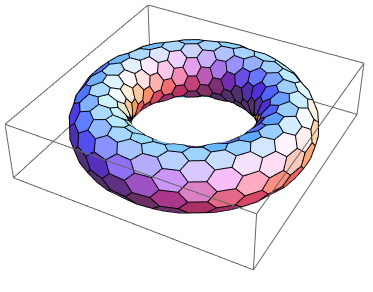
\includegraphics[width=0.75\textwidth]{images/test_image}
	\caption{H-Mode Confinement Time Scaling} ~\\
	\small This plot shows how well the ELMy H-Mode Scaling Law does for fitting $\tau_E$ to the ITER98 database of global tokamaks. For most values, the fit is at least 80\% accurate.
\end{figure}

The use of the ELMy H-Mode scaling law also brings up another subtlety in the field. To measure the movement of energy within a plasma, scaling relations are needed that correlate to specific modes of plasma behavior -- i.e. ones that can robustly be found by device technicians. Currently, people rank H-Mode scalings over L-Mode (because H stands for high confinement and L stands for low). However, people often seek out other modes that can reliably be found on other machines. These go by names like: I-Mode (i.e. intermediate confinement), Enhanced H-Mode, and Reversed Shear modes. \cite{imode,enhanced,shear}

Without going into too much detail, these alternate modes can be extremely valuable, as they often lead to cheaper reactor designs (than the ones made under H-Mode scaling). The problem, however, is often not finding a better performing mode on a single machine, but robustly finding it on other ones. This is important, because finding a mode on multiple machines is what allows new scaling relations to be produced and refined.\footnote{ In H-Mode and L-Mode's favor, they have been found on every machine that should see them. }

\section{Pricing a Fusion Reactor}

To compare tokamaks used as fusion reactors the obvious metrics to use are costs. ITER -- the second most expensive experiment today (only behind the LHC) -- has a history rich in countries backing out for high price tags and rejoining only when they are finally lowered. \cite{jeff} The problem is \$20B is a lot of money and 20 years is a long time. Moreover, approximating true costs becomes even trickier when designers the need to project (or neglect)  economies-of-scale for expensive components, e.g. the magnets.

As such, this paper adopts stand-ins for the conventional capital cost and cost-per-watt metrics. This is done for simplicity -- for both modeling reasons as well as conveying the two metrics to physicists. To begin, the relevant approximation for capital cost -- how much a tokamak reactor costs to build -- is the magnetic energy. \cite{griffiths}

\begin{equation}
	W_M \propto R^3 B^2
\end{equation}
\myequations{Magnetic Energy -- $W_M$}

In this magnetic energy proportion relation, the tokamak's major radius -- R -- is involved in a volumetric term and B is the strength (in Teslas) of the hooped shape magnetic field that lays nested within the plasma's shell (near its core). This quantity simply states that the two surefire ways to make a machine more expensive to build are: making it larger and using stronger magnets.

The next metric, the cost-per-watt, is defined by dividing the capital cost (i.e. the magnetic energy) by the main source of power output. In a tokamak, this is assumed to be fusion power, which relies on light elements (i.e. two Hydrogens) fusing into a heavier one (i.e. one Helium), thereby releasing enough energy to offset the expense of causing it to happen in the first place. Although fusion power will not be defined till later, it does highlight the fact that this measure of cost-per-watt actually has units of time!\footnote{As energy per unit watt has units of time (i.e seconds).}

The final piece of the costing puzzle is a duty factor that levelizes the comparison of pulsed and steady-state tokamaks. As pulsed machines may be off 20\% of the time, their fusion power output should be reduced by that percentage. This is accounted for in the duty factor, which is simply the ratio of the flattop -- the time when pulsed machines are approximately held at steady-state -- to the entire length of a pulsed. In pulsed machines, the entire pulse includes charging the inductive sources as well as flushing out the tokamak between runs. These non-flattop portions of time can last around thirty minutes (where the reactor makes no money). As steady-state machines lack these non-flattop portions, their duty factors are rightfully one.

Summarizing, the cost-per-watt coupled with the duty factor gives an ad hoc pricing metric, $C_W$, given by:

\begin{equation}
	\tcboxmath{
	C_W = \frac{W_M}{f_{Duty} \cdot P_F}
	}
\end{equation}
\myequations{Cost per Watt -- $C_W$}

It serves as a cornerstone for comparing the entire landscape of tokamak reactors -- whether they run in pulsed or steady-state operation. Although not a true engineering cost metric (i.e. in dollars per watt), it does provide an obvious physics meaning. Coupled with the magnetic energy stand-in for capital cost, profitable and inexpensive can now be easily pinpointed.

\section{Modeling a Fusion Reactor}

\# todo: bridge intro to rest of paper

\begin{enumerate}
	\item MIT campaign for High-Field Reactors
	\item Simple, quick model that matches higher dimensional codes
	\item Motivated by a desire for intuition over preciseness
	\item Desire to not explicitly solve elliptic integrals of the wrong kind in the complex plane
	\item Although cost stated as important, start over from square one
	\item Do steady-state and then pulsed and show they're basically the same
	\item the main conclusion is HTS is the best weapon we got
	\item jeffs quote: "by definition, mfe requires magnets"
	\item steady state : hts toroidal field magnets :: pulsed : hts central solenoid
	\item i.e. just use copper in steady-state no matter what
\end{enumerate}

%\end{document}
